%% TCC paper -- ACM small journal format, anonymous review version.
%% Layout of this project:
%%   main.tex            this file (preamble + section includes only)
%%   macros.tex          project-wide macros and listing/plot styles
%%   sections/*.tex      one file per section
%%   figures/*.tex       one TikZ/pgfplots file per figure (data in figures/data/)
%%   tables/*.tex        one file per table
%%   bib/references.bib  dblp-sourced bibliography (bib/fetch_dblp.py regenerates it)
%%   build.ps1           pdflatex + bibtex driver, writes to build/
\documentclass[acmsmall,screen,review,anonymous]{acmart}

%% Packages -------------------------------------------------------------------
\usepackage{booktabs}
\usepackage{multirow}
\usepackage{xspace}
\usepackage{listings}
\usepackage{subcaption}
\usepackage{tikz}
\usepackage{pgfplots}
\usepackage{pgfplotstable}
\pgfplotsset{compat=1.18}
\usepgfplotslibrary{groupplots}
\usetikzlibrary{positioning,arrows.meta,shapes.geometric,shapes.misc,fit,calc,backgrounds,matrix,decorations.pathreplacing}

%% Names -----------------------------------------------------------------------
\newcommand{\tool}{\textsc{Tcc}\xspace}
\newcommand{\tcompile}{\texttt{torch.compile}\xspace}
\newcommand{\code}[1]{\texttt{#1}}
\newcommand{\eg}{e.g.,\xspace}
\newcommand{\ie}{i.e.,\xspace}
\newcommand{\etal}{et al.\xspace}
\newcommand{\scs}{SCS\xspace}
\newcommand{\EZ}{$E_0$\xspace}
\newcommand{\EO}{$E_1$\xspace}
\newcommand{\ET}{$E_2$\xspace}
\newcommand{\ER}{$E_3$\xspace}

%% Answer boxes for research questions -----------------------------------------
\newcommand{\rqanswer}[2]{%
  \par\smallskip\noindent\fcolorbox{black!35}{black!4}{\parbox{\dimexpr\linewidth-2\fboxsep-2\fboxrule}{%
  \textbf{Answer to #1.} #2}}\par\smallskip}

%% Colour palette (Tol qualitative, colour-blind safe) ---------------------------
\definecolor{tolblue}{HTML}{0077BB}
\definecolor{tolcyan}{HTML}{33BBEE}
\definecolor{tolteal}{HTML}{009988}
\definecolor{tolorange}{HTML}{EE7733}
\definecolor{tolred}{HTML}{CC3311}
\definecolor{tolmagenta}{HTML}{EE3377}
\definecolor{tolgrey}{HTML}{BBBBBB}

%% Listings ---------------------------------------------------------------------
\lstdefinestyle{py}{
  language=Python,
  basicstyle=\ttfamily\footnotesize,
  keywordstyle=\color{tolblue}\bfseries,
  commentstyle=\color{black!55}\itshape,
  stringstyle=\color{tolred},
  numbers=left, numberstyle=\tiny\color{black!50}, numbersep=6pt,
  xleftmargin=1.6em, framexleftmargin=1.4em,
  frame=single, rulecolor=\color{black!25},
  showstringspaces=false, columns=fullflexible, keepspaces=true,
  escapeinside={(*@}{@*)},
  morekeywords={torch,compile,self,True,False,None}
}
\lstset{style=py}

%% pgfplots defaults --------------------------------------------------------------
\pgfplotsset{
  tccaxis/.style={
    width=\linewidth, height=4.4cm,
    tick label style={font=\scriptsize},
    label style={font=\footnotesize},
    legend style={font=\scriptsize, draw=black!30, fill=white, fill opacity=0.9, text opacity=1},
    axis line style={black!60}, tick style={black!60},
    ymajorgrids, grid style={black!10},
  }
}


%% Rights management information is irrelevant for a review copy.
\setcopyright{none}
\acmJournal{TOSEM}
\acmYear{2027}
\acmVolume{1}
\acmNumber{1}
\acmArticle{1}
\acmMonth{1}
\acmDOI{}
\settopmatter{printacmref=false}
\renewcommand\footnotetextcopyrightpermission[1]{}

\begin{document}

\title{Consistency Testing of AI Compiler Stacks by Varying the Compilation}

\author{Anonymous Author(s)}
\affiliation{\institution{Anonymous Institution}\country{Anonymous}}

\begin{abstract}
The same Python program can be compiled by \tcompile along several paths. Graph breaks are placed at positions
that depend on the call site, automatic differentiation is traced only when a gradient is required, loops are
vectorized only above a length threshold, execution may take place under a dispatch mode, autocast, or CUDA
graphs, and a program may be exported and packaged for deployment. Existing testing techniques for AI compiler
stacks vary the program and compile it along whichever path the harness takes, and they compare output
values. Consistency failures between eager and compiled execution, however, often occur where a rarely used
program feature meets a rarely taken path, and many of them do not change an output value.
This paper varies the compilation instead and treats its path as a test dimension. We identify four path factors that a harness can
enumerate and control one at a time: the position of graph breaks, the backend layer, the execution context,
and the artifact route from export to a packaged runtime. Together with program-side factors derived from the
source and from operator metadata, they form an execution matrix in which every difference from the reference
execution has one candidate cause. Executions are compared on seven observables (values against a
high-precision reference, metadata, object identity, exception type and routing, side effects, gradients, and
process survival), and layered execution names the compiler stage at which a difference first appears.
Applied to PyTorch~2.14 and nightly builds, the approach has produced 73 reports: 55 new issues, 15
issue comments, and 3 reports to a C++ compiler vendor. At the time of writing, 14 are fixed or have a fix under
review, 10 are confirmed, 48 await triage, and 1 was rejected. On a 185-program corpus that program-only
differential testing under three configurations had already covered, one path factor exposed two new defects; one
program-side factor exposed 134 operators that compute under \tcompile on dtypes their eager kernels reject.
Factor families for which no inconsistency was found are reported as well.
\end{abstract}


\begin{CCSXML}
<ccs2012>
<concept>
<concept_id>10011007.10011074.10011099.10011102.10011103</concept_id>
<concept_desc>Software and its engineering~Software testing and debugging</concept_desc>
<concept_significance>500</concept_significance>
</concept>
<concept>
<concept_id>10011007.10011006.10011041</concept_id>
<concept_desc>Software and its engineering~Compilers</concept_desc>
<concept_significance>500</concept_significance>
</concept>
<concept>
<concept_id>10010147.10010257</concept_id>
<concept_desc>Computing methodologies~Machine learning</concept_desc>
<concept_significance>300</concept_significance>
</concept>
</ccs2012>
\end{CCSXML}
\ccsdesc[500]{Software and its engineering~Software testing and debugging}
\ccsdesc[500]{Software and its engineering~Compilers}
\ccsdesc[300]{Computing methodologies~Machine learning}

\keywords{AI compiler stacks, torch.compile, consistency testing, varying the compilation, differential testing, metamorphic relation, graph breaks, JIT specialization}

\maketitle

\section{Introduction}
\label{sec:intro}

Deep learning (DL) programs are written, reviewed, and debugged as Python code, but they are increasingly
executed in another form. Since PyTorch~2, a call to \tcompile routes a model through bytecode-level graph
capture, functionalization and automatic-differentiation tracing, operator decomposition, loop-level lowering,
C++ or Triton code generation, guard-based specialization, and several caches~\cite{DBLP:conf/asplos/AnselYHGJVBBBBC24}.
Comparable pipelines exist in TVM~\cite{DBLP:conf/osdi/ChenMJZYSCWHCGK18}, XLA-backed TensorFlow~\cite{DBLP:conf/osdi/AbadiBCCDDDGIIK16}, MLIR-based
stacks~\cite{DBLP:conf/cgo/LattnerAB0DPRSV21}, and Triton~\cite{DBLP:conf/pldi/TilletKC19}; we call such a pipeline an \emph{AI compiler stack}. These systems are expected to produce an optimized artifact
that is semantically equivalent to eager execution, so that the Python source remains the single description of
what the program does.

This expectation can be violated without any visible sign in the source. An empirical study of \emph{toxic
compilation}\footnote{Reference withheld for double-anonymous review.} collected more than a thousand incidents
in which the produced artifact diverged from the reviewed source. We call their common outcome a
\emph{source--artifact consistency failure}: for the same program, input, and context, eager and compiled
execution differ in an observable way. Four of the defects reported in this paper illustrate the range. An
\code{OrderedDict.move\_to\_end} call inside a compiled function is dropped, so that an LRU cache maintained
next to the compiled step evicts the entry it has just used. An \code{IndexError} raised by a tensor operator
bypasses the \code{except} clause written for it. A generator that leaves the compiled region is returned as an
exhausted tuple iterator whose return value is \code{None}. The expression \code{x * 1} at the end of a graph
returns the input tensor itself, so that an in-place update of the result modifies the input.

Compiler testing has so far varied the \emph{program}. NNSmith~\cite{DBLP:conf/asplos/LiuLRTLPZ23}, NeuRI~\cite{DBLP:conf/sigsoft/0004PW023},
and HirGen~\cite{DBLP:conf/issta/MaS00C23} synthesize computation graphs; Tzer~\cite{DBLP:journals/pacmpl/LiuWYDZ22} and
MLIRSmith~\cite{DBLP:conf/kbse/WangCXLWSZ23} mutate intermediate representations; TorchProbe~\cite{DBLP:conf/aplas/SuGPS23} applies
semantics-preserving transformations to Python programs; FreeFuzz~\cite{DBLP:conf/icse/WeiDYZ22},
DeepREL~\cite{DBLP:conf/sigsoft/DengYWZ22}, and LLM-based fuzzers~\cite{DBLP:conf/issta/DengXPY023,DBLP:conf/icse/DengXYZY024} generate API
invocations. In all of these techniques a program is compiled along one path, the one the harness takes by
default. For \tcompile this leaves much of the compiler untested. Where TorchDynamo breaks the graph depends on
the call site; whether AOTAutograd participates depends on whether a gradient is needed; whether TorchInductor
emits a scalar or a vectorized loop depends on the tensor length; whether an operator takes a dedicated lowering
or a generic decomposition depends on its dtype; a \code{TorchDispatchMode}, autocast, or CUDA graphs change
which components run; export and ahead-of-time packaging replace the runtime. A defect on a path the harness
does not take remains undetected regardless of how many programs are generated.

The compilation itself can, however, be varied: its path can be enumerated and controlled one factor at a time. The statements after
which a graph break can be inserted, the backend layers that can be selected, the execution contexts that can
be entered, and the artifact routes that can be taken are switches exposed by the pipeline; their number is
small, their meaning is documented, and none of them is permitted to change the result of the program. The
program-side factors that change compiler behavior can be enumerated as well: a static analysis of the source
recovers the shapes, dtypes, scalars, and flags a compilation site reads, and operator metadata lists the dtypes
and sample shapes each operator supports. Treating both groups as test dimensions, holding one fixed and
changing the other by one factor at a time, yields tests in which every difference has a single candidate cause.
A path factor is a semantics-preserving change to how the program is compiled, so the eager result is the
expected outcome of a metamorphic relation~\cite{DBLP:journals/csur/ChenKLPTTZ18}; the relation is the same for
every factor, and the design effort goes into the choice of observables that are compared.

We implement this approach in \tool. Section~\ref{sec:approach} defines the factor model, the one-factor
execution matrix, an oracle over seven observables (values against a float64 or multi-precision reference,
dtype and shape and stride, object identity and aliasing, exception type and its routing to a handler, side
effects on inputs and external state, gradients, and process survival), and layered localization, which names
the stage at which a difference first appears. Section~\ref{sec:analyzers} describes how the path factors are
realized on \tcompile and how program-side factors are drawn from the source and from operator metadata.

\paragraph{Results.} Reports filed against PyTorch~2.14 and nightly builds during the study number 73: 55 new
issues, 15 comments that add members or root causes to existing issues, and 3 reports to the vendor of the C++
compiler that TorchInductor uses on Windows. At the time of writing, 14 are fixed or have a fix under review, 10
are confirmed by maintainers or reproduced by other contributors, 48 await triage, and 1 was judged expected
behavior. A corpus of 185 programs that program-only differential testing under three configurations had already
covered yielded two new Dynamo defects when one path factor, the position of graph breaks, was added. One
metadata-derived factor exposed 134 operators that compute under \tcompile on dtypes their eager kernels
reject. Of the 58 findings attributable to the compile pipeline, 39 are detectable only through an observable
other than the output value. Guards, caches, compile composition, autocast, higher-order operators, custom
operators, and the numerical behavior of the export path were consistent in every configuration we tried.

\paragraph{Contributions.}
\begin{itemize}
  \item Varying the compilation as a dimension of consistency testing, with a set of path factors that a
        harness can enumerate and control (graph-break position, backend layer, execution context, artifact
        route), and evidence that program-only testing does not reach the defects on rarely taken paths
        (Sections~\ref{sec:approach}, \ref{sec:analyzers}, \ref{sec:rq1}).
  \item A one-factor execution matrix over program-side and path-side factors and an oracle over seven
        observables, which make every difference attributable and make side-effect, identity,
        exception-routing, and process-level failures detectable (Sections~\ref{sec:approach}, \ref{sec:rq3}).
  \item An evaluation on injected faults, historical issues, and current PyTorch builds, with 73 reports
        classified by maintainer response and by root-cause location, and negative results that state where
        consistency holds (Section~\ref{sec:eval}).
\end{itemize}

\section{Background and Motivation}
\label{sec:background}

\subsection{The \tcompile Stack}
\label{sec:stack}

\tcompile wraps a Python callable and defers compilation to the first call~\cite{DBLP:conf/asplos/AnselYHGJVBBBBC24}. Four layers then
transform the program. \emph{TorchDynamo} symbolically evaluates CPython bytecode, models Python objects with
variable trackers, extracts an FX graph~\cite{DBLP:conf/mlsys/ReedDHUA22} of tensor operations, and installs \emph{guards}: predicates
over input metadata, Python values, and global state under which the captured graph may be reused. Code that
Dynamo cannot model causes a graph break and falls back to the interpreter. \emph{AOTAutograd} traces the graph
with \emph{fake tensors} that carry only metadata, removes mutation and aliasing through functionalization,
and records a joint forward/backward graph. A \emph{decomposition} table rewrites several hundred ATen operators
into a smaller primitive set, and \emph{meta kernels} compute output shapes, dtypes, and strides without data.
\emph{TorchInductor} lowers the primitives to a loop-level IR, fuses them, and generates C++/OpenMP code for CPUs
or Triton kernels~\cite{DBLP:conf/pldi/TilletKC19} for GPUs. Compiled code is kept in an in-memory cache keyed by guards and in
on-disk caches keyed by graph and configuration hashes; the same graph can also be exported ahead of time and
packaged by AOTInductor.

Each layer can be selected in isolation through the \code{backend} argument, which \tool exploits for
localization: \code{backend="eager"} executes the graph captured by Dynamo with eager kernels (\EO),
\code{"aot\_eager"} adds AOTAutograd and decompositions (\ET), and \code{"inductor"} adds lowering and code
generation (\ER). Plain eager execution is \EZ.

\subsection{Source--Artifact Consistency}
\label{sec:definition}

Let $f$ be a Python function, $x$ an input, and $c$ an execution context that fixes tensor metadata, Python-level
values, global state, and compiler options. $E(f,x,c)$ denotes eager execution and $C(f,x,c)$ compiled execution.
We compare executions through the observation
\[
\mathit{Obs}(r)=\langle \mathit{value},\ \mathit{metadata},\ \mathit{identity},\ \mathit{exception},\ \mathit{state},\ \mathit{gradient},\ \mathit{process}\rangle ,
\]
where metadata covers shape, dtype, stride, device, and layout; identity records whether an output is an input
object or shares its storage; exception covers the type of a raised exception and whether a handler in the
program received it; state is the post-state of inputs, module buffers, and Python objects the program can
reach; and process records whether the interpreter survived. The compiler is \emph{consistent} on $(f,x,c)$ if
$\mathit{Obs}(E(f,x,c)) \approx \mathit{Obs}(C(f,x,c))$, where $\approx$ is equality except for a dtype-aware
floating-point tolerance on values and gradients. For caches we additionally compare a cold compilation in
context $c_2$ with a warm execution that first compiles under $c_1$:
$C_{\mathit{cold}}(f,x,c_2)$ versus $C_{\mathit{warm}}(f,x,c_1\!\rightarrow\!c_2)$. If eager and cold agree but warm
differs, the failure is attributed to specialization or cache reuse rather than to code generation. The context
$c$ has two parts: the program-side part (metadata, values, state) that the program can read, and the
\emph{compilation path} (graph-break positions, backend layer, execution context, artifact route) that the
program cannot observe and that must therefore never change $\mathit{Obs}$. This paper varies both.

\subsection{Motivating Examples}
\label{sec:motivation}

%% Figure: two motivating defects, each with its layer outcome strip.
\newcommand{\layercell}[3]{% #1 label, #2 colour, #3 text
  \node[draw=black!40, fill=#2, minimum width=1.5cm, minimum height=0.62cm, font=\scriptsize, align=center,
        inner sep=1pt] (#1) {#3};}
\begin{figure}[t]
\centering
\begin{minipage}[t]{0.485\linewidth}
\begin{lstlisting}
import random, torch

def augment(x):
    idx = [0, 1, 2, 3]
    random.shuffle(idx)  # Python state
    return x[idx]

g = torch.compile(augment)
x = torch.arange(4.)
g(x); g(x); g(x)   # same order each time
\end{lstlisting}
\centering
\begin{tikzpicture}[node distance=0pt]
  \layercell{a0}{tolteal!18}{\EZ eager\\varies}
  \node[right=2pt of a0] (s1) {};
  \begin{scope}[shift={(1.62,0)}]\layercell{a1}{tolred!22}{\EO Dynamo\\frozen}\end{scope}
  \begin{scope}[shift={(3.24,0)}]\layercell{a2}{tolred!22}{\ET AOT\\frozen}\end{scope}
  \begin{scope}[shift={(4.86,0)}]\layercell{a3}{tolred!22}{\ER Inductor\\frozen}\end{scope}
\end{tikzpicture}
\subcaption{\code{random.shuffle} is evaluated once at trace time: divergence enters at graph capture and is
visible only when the artifact is reused.}
\end{minipage}\hfill
\begin{minipage}[t]{0.485\linewidth}
\begin{lstlisting}
import torch

def stats(x):
    return torch.var_mean(x, correction=1)

x = torch.randn(0)        # shape[0] = 0
stats(x)                  # (nan, nan)
torch.compile(stats)(x)   # (nan, 0.)
# same for std_mean, float16, (0, 1),
# dynamic=True, and AOTInductor
\end{lstlisting}
\centering
\begin{tikzpicture}[node distance=0pt]
  \layercell{b0}{tolteal!18}{\EZ eager\\(nan, nan)}
  \begin{scope}[shift={(1.62,0)}]\layercell{b1}{tolteal!18}{\EO Dynamo\\(nan, nan)}\end{scope}
  \begin{scope}[shift={(3.24,0)}]\layercell{b2}{tolteal!18}{\ET AOT\\(nan, nan)}\end{scope}
  \begin{scope}[shift={(4.86,0)}]\layercell{b3}{tolred!22}{\ER Inductor\\(nan, 0.)}\end{scope}
\end{tikzpicture}
\subcaption{A boundary value of \code{x.shape[0]} makes Inductor fabricate a mean of zero: $E_0{=}E_1{=}E_2{\neq}E_3$
localizes the defect to code generation.}
\end{minipage}
\caption{Two source--artifact consistency failures found by \tool in PyTorch~2.14. Each strip shows the outcome
on eager execution and on the three compiled layers used for localization.}
\label{fig:motivation}
\end{figure}


Figure~\ref{fig:motivation} shows two defects found by \tool in PyTorch~2.14 that illustrate why neither graph
diversity nor an output-only oracle is sufficient.

\paragraph{A Python-semantics failure.} In Figure~\ref{fig:motivation}a, eager execution advances the global
random state, so consecutive calls return different permutations. Under \tcompile every call returns the
permutation drawn during tracing. The outcome is identical for \EO, \ET, and \ER, which places the divergence
in graph capture: Dynamo evaluates \code{random.shuffle} at trace time and embeds the result as a constant. No
tensor operator is wrong, no exception is raised, and a single-call differential test passes; the defect is
visible only when the same artifact is \emph{reused}, which is the sequence dimension of our test model.

\paragraph{A code-generation failure on a boundary shape.} In Figure~\ref{fig:motivation}b,
\code{torch.var\_mean} on an empty tensor returns \code{(nan, nan)} in eager mode and under \EO and \ET, but
\code{(nan, 0.)} under Inductor. The mean component is a fabricated zero. The trigger is a boundary value of the
factor \code{x.shape[0]}, and the layer pattern $E_0{=}E_1{=}E_2{\neq}E_3$ assigns the defect to Inductor's
reduction code. The operator is covered by PyTorch's own test suite, but not with this shape under the compiled
path.

\paragraph{Observations.} Both failures arise where a \emph{legal but uncommon context} meets a compilation
path, both are invisible to a generator that varies only graph topology, and they differ in layer, observable,
and trigger, which calls for a systematic model of context factors instead of one specialized oracle.

\section{The \tool Approach}
\label{sec:approach}

%% Figure: overview of the approach (four phases + factor-family analyzers).
\begin{figure}[t]
\centering
\resizebox{\linewidth}{!}{%
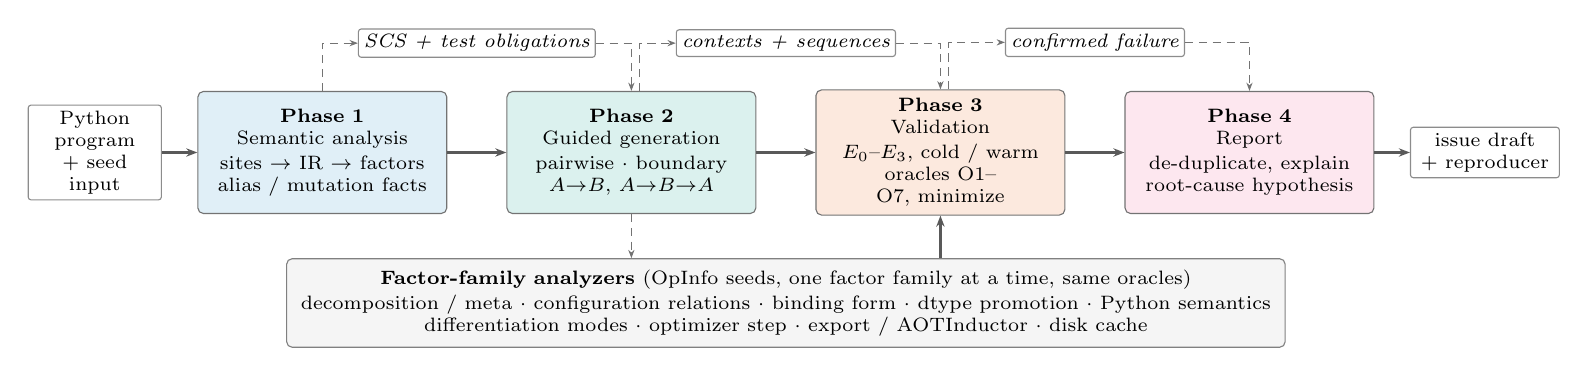
\begin{tikzpicture}[
    font=\scriptsize,
    phase/.style={draw=black!55, rounded corners=2pt, fill=#1, align=center, minimum height=1.55cm,
                  text width=2.95cm, inner sep=3pt},
    art/.style={draw=black!45, fill=white, align=center, font=\scriptsize\itshape, inner sep=2pt,
                rounded corners=1pt},
    flow/.style={-{Stealth[length=4pt]}, thick, black!65},
    side/.style={-{Stealth[length=3pt]}, black!55, densely dashed},
]
  %% phases
  \node[phase=tolblue!12] (p1) {\textbf{Phase 1}\\Semantic analysis\\[1pt]
        sites $\rightarrow$ IR $\rightarrow$ factors\\alias / mutation facts};
  \node[phase=tolteal!14, right=0.75cm of p1] (p2) {\textbf{Phase 2}\\Guided generation\\[1pt]
        pairwise $\cdot$ boundary\\$A{\rightarrow}B$, $A{\rightarrow}B{\rightarrow}A$};
  \node[phase=tolorange!16, right=0.75cm of p2] (p3) {\textbf{Phase 3}\\Validation\\[1pt]
        $E_0$--$E_3$, cold / warm\\oracles O1--O7, minimize};
  \node[phase=tolmagenta!12, right=0.75cm of p3] (p4) {\textbf{Phase 4}\\Report\\[1pt]
        de-duplicate, explain\\root-cause hypothesis};
  %% artifacts between phases
  \node[art, above=0.42cm of $(p1.north)!0.5!(p2.north)$] (scs) {SCS + test obligations};
  \node[art, above=0.42cm of $(p2.north)!0.5!(p3.north)$] (tests) {contexts + sequences};
  \node[art, above=0.42cm of $(p3.north)!0.5!(p4.north)$] (fail) {confirmed failure};
  \draw[flow] (p1) -- (p2); \draw[flow] (p2) -- (p3); \draw[flow] (p3) -- (p4);
  \draw[side] (p1.north) |- (scs.west); \draw[side] (scs.east) -| (p2.north);
  \draw[side] ([xshift=3pt]p2.north) |- (tests.west); \draw[side] (tests.east) -| (p3.north);
  \draw[side] ([xshift=3pt]p3.north) |- (fail.west); \draw[side] (fail.east) -| (p4.north);
  %% inputs / outputs
  \node[art, left=0.45cm of p1, text width=1.55cm, font=\scriptsize] (in) {Python program\\+ seed input};
  \node[art, right=0.45cm of p4, text width=1.75cm, font=\scriptsize] (out) {issue draft\\+ reproducer};
  \draw[flow] (in) -- (p1); \draw[flow] (p4) -- (out);
  %% analyzers lane
  \node[draw=black!50, rounded corners=2pt, fill=black!4, below=0.55cm of $(p2.south)!0.5!(p3.south)$,
        text width=12.4cm, align=center, inner sep=4pt] (an)
        {\textbf{Factor-family analyzers} (OpInfo seeds, one factor family at a time, same oracles)\\[1pt]
         decomposition / meta $\cdot$ configuration relations $\cdot$ binding form $\cdot$ dtype promotion $\cdot$
         Python semantics\\ differentiation modes $\cdot$ optimizer step $\cdot$ export / AOTInductor $\cdot$ disk cache};
  \draw[flow] (an.north -| p3.south) -- (p3.south);
  \draw[side] (p2.south) -- (an.north -| p2.south);
\end{tikzpicture}}
\caption{Overview of \tool. Phase~1 derives the context factors a compilation site reads; Phase~2 changes one
factor at a time; Phase~3 compares eager and layered compiled executions, cold and warm; Phase~4 packages
confirmed failures. The analyzers reuse Phases~3 and~4 for factor families that are not visible in user code.}
\label{fig:overview}
\end{figure}


Figure~\ref{fig:overview} gives an overview. A compiled execution is determined by three things: the program,
its input, and the path the compiler takes. \tool derives \emph{factors} for the first two from the source and
from operator metadata, derives factors for the third from the structure of the pipeline, and executes a matrix
in which each test differs from a reference execution in exactly one factor. A fixed oracle over seven
observables decides whether the difference is a failure, and layered execution names the stage at which it
appears.

\subsection{Factor Model}
\label{sec:factors}

\paragraph{Program-side factors from the source.} \tool locates \emph{compilation sites}, the boundaries at
which Python code enters the compiler (calls and decorators of \tcompile and project-specific wrappers), and
lowers every function reachable from a site into a small dependency IR with data, control, alias, and state
edges (Figure~\ref{fig:factors}). A context attribute becomes a \emph{semantic factor} of the site when a
backward slice from a \code{Return}, \code{Raise}, \code{Mutation}, or \code{StateWrite} node reaches a read of
that attribute: the rank, shape, stride, dtype, device, contiguity, and \code{requires\_grad} of a tensor
parameter; the value of a scalar, flag, string, or container; a global or closure variable. Comparisons and
modulo tests on integer factors yield boundary values (for \code{x.shape[0] >= 32} the values 32, 31, 33);
shape--index chains are recovered through constant offsets; writes through views yield alias and mutation facts
that determine which inputs must be built as views or overlapping buffers. The factors of a
site, with the backend and compile flags, form its \emph{Semantic Context Signature} (\scs); attributes the
program never reads are pruned. The analysis is syntactic and takes about 30~ms for our 29-program corpus.

%% Figure: from a small program to its dependency graph, factors, and obligations.
\begin{figure}[t]
\centering
\begin{minipage}[c]{0.37\linewidth}
\begin{lstlisting}
def f(x, use_fast):
    n = x.shape[0]
    y = x.view(-1)
    if use_fast and n >= 32:
        y[n - 1] += 1
    return x.sum(dtype=x.dtype)
\end{lstlisting}
\end{minipage}\hfill
\begin{minipage}[c]{0.61\linewidth}
\centering
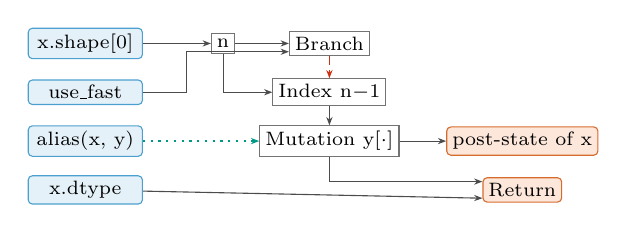
\begin{tikzpicture}[
    font=\scriptsize, x=1cm, y=0.62cm,
    attr/.style={draw=tolblue!70, fill=tolblue!10, rounded corners=1.5pt, inner sep=2pt, minimum width=1.45cm},
    ir/.style={draw=black!55, fill=white, inner sep=2pt},
    obs/.style={draw=tolorange!90!black, fill=tolorange!18, rounded corners=1.5pt, inner sep=2pt},
    d/.style={-{Stealth[length=3pt]}, black!70},
    c/.style={-{Stealth[length=3pt]}, tolred, densely dashed},
    a/.style={-{Stealth[length=3pt]}, tolteal, thick, dotted},
]
  \node[attr] (shape) at (0,3) {x.shape[0]};
  \node[attr] (flag)  at (0,2) {use\_fast};
  \node[attr] (alias) at (0,1) {alias(x, y)};
  \node[attr] (dtype) at (0,0) {x.dtype};
  \node[ir] (n)   at (1.75,3) {n};
  \node[ir] (br)  at (3.1,3) {Branch};
  \node[ir] (idx) at (3.1,2) {Index n$-$1};
  \node[ir] (mut) at (3.1,1) {Mutation y[$\cdot$]};
  \node[obs] (state) at (5.55,1) {post-state of x};
  \node[obs] (ret)   at (5.55,0) {Return};
  \draw[d] (shape) -- (n); \draw[d] (n) -- (br);
  \draw[d] (n.south) |- (idx.west);
  \draw[d] (flag.east) -- ++(0.55,0) |- ([yshift=-3pt]br.west);
  \draw[c] (br) -- (idx); \draw[d] (idx) -- (mut);
  \draw[a] (alias) -- (mut); \draw[d] (mut) -- (state);
  \draw[d] (mut.south) |- ([yshift=3pt]ret.west);
  \draw[d] (dtype) -- ([yshift=-3pt]ret.west);
\end{tikzpicture}
\end{minipage}

\vspace{3pt}
{\scriptsize
\begin{tabular}{@{}llll@{}}
\toprule
Factor & Constraint values & Oracles & Execution \\
\midrule
\code{x.shape[0]} & 32, 31, 33 (predicate); $n{-}1$ (index bound) & value, exception & cold \\
\code{use\_fast} & True, False, on each side of $n \geq 32$ & value, mutation & cold + warm \\
\code{x.dtype} & float16, float32, float64, bfloat16 & value, metadata & cold + warm \\
\code{alias(x, y)} & contiguous, non-contiguous, overlapping view & mutation, alias & cold \\
\bottomrule
\end{tabular}}
\caption{Phase~1 on a small function. Solid edges are data dependencies, dashed edges control dependencies, dotted
edges alias dependencies. Attributes that reach an observable (orange) become semantic factors; each factor yields
a test obligation. Attributes the function never reads, such as \code{x.stride}, are pruned.}
\label{fig:factors}
\end{figure}


\paragraph{Program-side factors from operator metadata.} For operator-level testing the source is a single
call, and the informative factors come from PyTorch's OpInfo database, which lists for about 700 operators the
supported dtypes, sample inputs, and reference implementations. \tool derives three factor families from it:
\emph{boundary values}, which replace sample data by infinities, NaN, the dtype extremes, values next to
singularities (\code{nextafter(1, 0)} for inverse functions, $\pi/2$, $1 \pm \epsilon$) and magnitudes near
overflow, in tensors long enough to reach vectorized code; \emph{unsupported dtypes}, which cast a sample to a
dtype the eager kernel rejects; and \emph{dtype pairs} for binary operators. Each family is a change of one
factor of one call; the operator and the shape stay fixed.

\paragraph{Path-side factors from the pipeline.} The compilation path is determined by choices the pipeline
exposes and documents as semantics-preserving. \tool treats four of them as factors.
\begin{itemize}
  \item \emph{Graph-break position.} A call to \code{torch.\_dynamo.graph\_break()} splits the captured graph
        and makes Dynamo generate a resume function that carries locals, side effects, exception state, and
        live objects across the break. Inserting the call after any statement must not change the result.
  \item \emph{Backend layer.} \code{backend="eager"} executes the captured graph with eager kernels,
        \code{"aot\_eager"} adds AOTAutograd and decompositions, \code{"inductor"} adds lowering and code
        generation. Each layer is a semantics-preserving refinement of the previous one.
  \item \emph{Execution context.} A \code{TorchDispatchMode} that only forwards calls, autocast, \code{dynamic=True},
        \code{fullgraph}, compile composition (a compiled function calling another, \code{compile(compile(f))}),
        and CUDA-graph or autotuning modes change which components run without changing what the program
        means.
  \item \emph{Artifact route.} \code{torch.export}, its serialization round trip, AOTInductor packaging and
        loading, and the lifetime of the loaded runner replace the just-in-time runtime by a deployed one.
\end{itemize}
Every path factor has a reference execution in which the factor takes its default value, and the expected
outcome is that the observables do not change. In the terminology of metamorphic testing~\cite{DBLP:journals/csur/ChenKLPTTZ18,DBLP:journals/tse/SeguraFSC16},
each path factor is a semantics-preserving transformation of the compilation, the eager run is the source
test case, and observable equality is the relation. Because the relation is the same for all factors, one
oracle serves the whole matrix. Program-side factors are transformations of the input instead of
the compilation, but they are tested against the same relation.

\subsection{One-Factor Execution Matrix}
\label{sec:matrix}

\paragraph{Seeds.} \tool does not invent programs. A seed is a valid call of a compilation site, obtained from
the function signature, from recorded calls, from reproducer scripts, from OpInfo samples, or from a corpus of
small Python programs written for the features Dynamo models itself (the \code{random} module, exceptions and
handlers, generators and their protocol, context managers, containers and their mutation, tensor subclasses;
274 programs at the time of writing). Programs in the corpus are added by mechanism: when a factor exposes a
defect in one construct, programs that exercise the same mechanism in other constructs are written before the
sweep is repeated (Section~\ref{sec:rq1}).

\paragraph{Single-factor variants.} For each obligation derived from the \scs, \tool builds contexts that
differ from the seed in exactly one program-side factor, drawing values round-robin over obligations so that a
small budget covers every factor once before any factor twice. For each path factor it builds the variant that
changes only that factor: the corpus program with a graph break after every statement, the same call under
another backend layer, inside a dispatch mode, or through the export route. A context in which eager execution
of the mutated input raises is kept when the exception is the behavior under test; programs that eager
execution rejects and the compiler accepts are a defect class of their own (Section~\ref{sec:rq3}).

%% Figure: execution matrix as a sequence diagram (cold vs warm, return trip).
\begin{figure}[t]
\centering
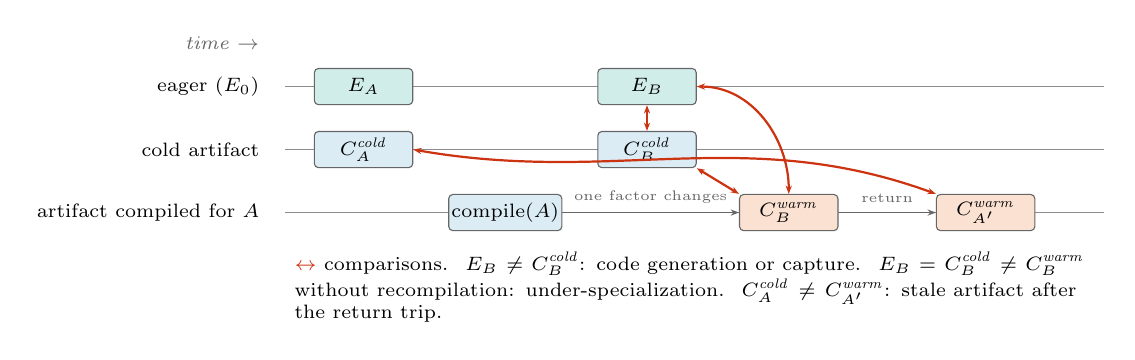
\begin{tikzpicture}[
    font=\scriptsize,
    lane/.style={black!45, thin},
    run/.style={draw=black!60, fill=#1, rounded corners=1.5pt, minimum width=1.25cm, minimum height=0.46cm,
                inner sep=1pt},
    cmp/.style={{Stealth[length=3pt]}-{Stealth[length=3pt]}, tolred, thick},
]
  %% lanes
  \foreach \y/\lab in {0/{eager (\EZ)}, -0.8/{cold artifact}, -1.6/{artifact compiled for $A$}} {
    \node[anchor=east] at (-0.2,\y) {\lab};
    \draw[lane] (0,\y) -- (10.4,\y);
  }
  \node[anchor=east, font=\scriptsize\itshape, black!60] at (-0.2,0.55) {time $\rightarrow$};
  %% eager runs
  \node[run=tolteal!18] (ea) at (1.0,0) {$E_A$};
  \node[run=tolteal!18] (eb) at (4.6,0) {$E_B$};
  %% cold runs
  \node[run=tolblue!14] (ca) at (1.0,-0.8) {$C_A^{\mathit{cold}}$};
  \node[run=tolblue!14] (cb) at (4.6,-0.8) {$C_B^{\mathit{cold}}$};
  %% warm sequence
  \node[run=tolblue!14] (wa) at (2.8,-1.6) {compile($A$)};
  \node[run=tolorange!22] (wb) at (6.4,-1.6) {$C_B^{\mathit{warm}}$};
  \node[run=tolorange!22] (wa2) at (8.9,-1.6) {$C_{A'}^{\mathit{warm}}$};
  \draw[-{Stealth[length=3pt]}, black!60] (wa) -- node[above, font=\tiny] {one factor changes} (wb);
  \draw[-{Stealth[length=3pt]}, black!60] (wb) -- node[above, font=\tiny] {return} (wa2);
  %% comparisons
  \draw[cmp] (eb) -- (cb);
  \draw[cmp] (cb.south east) -- (wb.north west);
  \draw[cmp] (eb.east) to[out=0, in=90] (wb.north);
  \draw[cmp] (ca.east) to[out=-10, in=160] (wa2.north west);
  %% verdict legend
  \node[anchor=west, align=left, font=\scriptsize, text width=10.2cm] at (0,-2.55)
    {\textcolor{tolred}{$\leftrightarrow$} comparisons.\;
     $E_B \neq C_B^{\mathit{cold}}$: code generation or capture.\;
     $E_B = C_B^{\mathit{cold}} \neq C_B^{\mathit{warm}}$ without recompilation: under-specialization.\;
     $C_A^{\mathit{cold}} \neq C_{A'}^{\mathit{warm}}$: stale artifact after the return trip.};
\end{tikzpicture}
\caption{Execution matrix for two contexts $A$ and $B$ that differ in one semantic factor. Recompilations are
counted exactly, so each verdict is tied to an observed cache decision.}
\label{fig:sequence}
\end{figure}


\paragraph{Context sequences.} Guards and caches are exercised by the execution matrix of
Figure~\ref{fig:sequence}: for contexts $A$ and $B$ that differ in one factor, eager and cold-compiled runs of
both, a warm run of $B$ on the artifact compiled for $A$, and the return trip. The comparison of $E_B$ with
$C_B^{\mathit{cold}}$ and with $C_B^{\mathit{warm}}$ separates code generation from under-specialization, and
the return trip exposes incorrect invalidation. Recompilations are counted through Dynamo's frame counters with
disk caches disabled.

\subsection{Oracle}
\label{sec:oracle}

\begin{table}[t]
\caption{The seven observables compared by \tool and the mechanisms each one exposes. Cold and warm executions
of Figure~\ref{fig:sequence} are compared on every observable.}
\label{tab:oracles}
\footnotesize
\begin{tabular}{@{}lp{5.1cm}p{6.0cm}@{}}
\toprule
Observable & Compared observation & Typical mechanism exposed \\
\midrule
O1 Value & scalars, tensors, nested containers; float64 or 30-digit reference with a dtype-aware noise floor; NaN/Inf pattern; sign of zero & wrong generated loop, unstable fused reduction, fabricated value on an empty reduction, vector polynomial with absolute-only accuracy \\
O2 Metadata & shape, dtype, stride, device, layout & wrong dtype promotion in a lowering, lost \code{channels\_last}, ignored \code{device=} \\
O3 Identity & output \emph{is} an input; storage sharing between inputs and outputs & no-op elimination that returns the input object, view replaced by a copy, generator replaced by an iterator \\
O4 Exception & raised or not; innermost exception type; whether the program's handler ran & missing validation, internal assertion, compile-only failure, exception that bypasses \code{except} \\
O5 State & post-state of inputs, module buffers, reachable Python objects; count of external effects & dropped or reordered in-place update, dropped container mutation, side effect replayed twice \\
O6 Gradient & input and parameter gradients against a higher-precision reference & wrong backward after tracing, lost in-place check, zero gradient from underflow \\
O7 Process & exit code and signal of the child process & native crash, hang, runtime destroyed while its threads run \\
\bottomrule
\end{tabular}
\end{table}


Table~\ref{tab:oracles} lists the seven observables. Values and gradients are compared against a reference,
not against a fixed tolerance: every test is also executed in eager mode with floating-point inputs promoted to
float64, and for elementary functions against a 30-digit multi-precision library, and a compiled result is
flagged only if its distance to the reference exceeds the distance of the eager result by a dtype-dependent
factor, or if its NaN/Inf pattern or the sign of a zero differs. This rule accepts compiled results that are
more accurate than eager execution and rejects one-ULP differences of re-associated reductions. Metadata covers
dtype, shape, stride, device, and layout. Identity records whether an output \emph{is} an input or shares its
storage, because a compiler that returns the input object where eager execution returns a copy changes the
meaning of every later in-place update. The exception observable compares the innermost exception of the
\code{\_\_cause\_\_} chain and, when the program contains a handler, whether the handler ran. State covers the
post-state of inputs, module buffers, and Python objects reachable from the program (lists, dictionaries,
generators), and the count of external effects such as printed lines. The process observable records exit codes
and signals, since several findings terminate the interpreter.

\subsection{Localization, Confirmation, and Reports}
\label{sec:phase3}

A failing test is re-executed on the backend layers \EO--\ER (and on the Triton path when a GPU is present).
The first layer that disagrees with its predecessor names the suspected stage: graph capture, functionalization
and decomposition, or code generation; a disagreement that appears only in a warm run names specialization or
cache reuse; a disagreement that also appears without \tcompile, for example under a forwarding dispatch mode
or in the eager kernel that the compiled path calls, is attributed \emph{outside} the pipeline and reported as
such. A candidate must survive a deterministic rerun with a fixed seed, a check that eager execution is
deterministic on the input, and a rerun in a fresh interpreter; every work item of a sweep runs in a child
process so that native crashes become findings instead of ending the sweep. Inputs are then minimized over
rank, shape, values, container sizes, flags, and arguments, and the program is minimized by deleting statements
outside the static slice of the triggering factor. A confirmed failure is emitted with the minimal reproducer, the observations on every layer, the factor that
triggered it, and, where the generated code allows it, the responsible source location and a candidate patch.
Likely duplicates are annotated, never filed; submission remains a human decision.

\section{Realizing the Factors on \tcompile}
\label{sec:analyzers}

Each factor family of Section~\ref{sec:factors} is realized as an \emph{analyzer}: a sweep that takes seeds
from one source, changes one factor, and reuses the oracle, confirmation, and reporting of
Section~\ref{sec:phase3}. Table~\ref{tab:analyzers} lists them with the scale of one sweep on PyTorch~2.14.
The path-side analyzers are new; the program-side ones extend the metadata-driven sweeps of earlier
differential testers with boundary values and unsupported dtypes.

\begin{table}[t]
\caption{Analyzers: the factor that is varied, the reference the result is compared with, and the scale of one
sweep on PyTorch~2.14 (CPU unless noted). Path-side analyzers vary how the program is compiled; program-side
analyzers vary the input or the operator call.}
\label{tab:analyzers}
\scriptsize
\setlength{\tabcolsep}{4pt}
\begin{tabular}{@{}lp{3.05cm}p{4.9cm}p{4.3cm}@{}}
\toprule
Side & Analyzer & Varied factor & Scale of one sweep \\
\midrule
path & graph-break position & a break after every statement (top level or nested), by \code{graph\_break}, \code{disable}, or \code{print}; three backends; \code{dynamic} & 274 programs, 660--816 insertion points, 6~min per backend \\
path & backend layer, context & \code{eager} / \code{aot\_eager} / \code{inductor}; forwarding dispatch mode (forward and gradients); autocast; 17 compile compositions & 955 differentiable op--dtype pairs; 530 ops $\times$ 2 autocast dtypes; 14 programs $\times$ 25 compositions \\
path & artifact route & \code{export} + serialize + load; AOTInductor package + load; runner destroyed after a run; CUDA-graph output reuse (19 patterns) & 520 ops (CPU), 19 patterns (T4) \\
path & context sequences & one factor changed between two calls of one artifact; return trip; cross-process disk cache & 26 switches, 29 cache cases \\
\midrule
program & boundary values & inf, NaN, extremes, near-singular and near-overflow values in vector-length tensors; \code{dynamic}; multi-precision reference for 44 unary and 23 binary functions & 1{,}203--1{,}345 op--dtype pairs per platform (CPU, T4) \\
program & unsupported dtypes & every dtype the eager kernel rejects & 1{,}345 pairs (CPU), 1{,}303 (T4) \\
program & dtype pairs, scalars & $8{\times}8$ dtype pairs in 4 argument forms; 11 binding forms of a scalar & 17{,}664 cases; 386 ops \\
program & source factors (\scs) & one semantic factor of a compilation site at a time; boundary values from predicates & 29 corpus programs, 114 obligations \\
program & Python corpus & 274 programs of Dynamo-modeled Python features, two calls each & 3 backends $\times$ 2 shape modes \\
program & decomposition, differentiation & Inductor decomposition executed eagerly; backward, complex, forward-mode, \code{vmap}; 11 optimizers & 576 ops, 11{,}911 variants; 327--678 ops per mode \\
\bottomrule
\end{tabular}
\end{table}


\paragraph{Graph-break position.} The corpus programs are rewritten at the syntax-tree level so that
\code{torch.\_dynamo.graph\_break()} follows every statement, either at the top level of the function or also
inside loop, conditional, \code{with}, and \code{try} bodies; nested function definitions are left intact and
closures are re-bound to the original cells so that the rewritten function sees the same state. The rewritten
program is compared with eager execution and with the un-rewritten compiled program in the same process, so
that the report lists the divergences the break \emph{added}. Three variants replace the break by a statement
with the same effect through a different mechanism: a call to a function wrapped in Dynamo's \code{disable}
decorator, a \code{print}, and a Python side effect on external state; the first two force a break with and without an
observable effect, the third produces no break and tests side-effect replay alone.

\paragraph{Backend layer and execution context.} The same seed is executed with \code{backend} set to each layer,
with \code{dynamic=True}, under a \code{TorchDispatchMode} whose \code{\_\_torch\_dispatch\_\_} only forwards
the call (the mode is entered by the compile runtime itself, so a difference here means that the compiled
program computes under a mode the user never wrote), under autocast, and under compositions of
\tcompile that occur in application code (a compiled function calling another, \code{compile(compile(f))},
\code{fullgraph}, a warm-up in \code{no\_grad} before a call with gradients, two backends on one function).
For differentiable operators the sweep also compares input gradients. Every difference is confirmed without
\tcompile where possible, which is how three findings were attributed to the dispatch machinery rather than to
the compiler.

\paragraph{Artifact route.} Each OpInfo sample is exported, serialized and deserialized, and executed; packaged
with AOTInductor, loaded, and executed; and the loaded runner is destroyed while its outputs are alive and
before the OpenMP worker threads of its last kernel have parked. Outputs are compared with eager execution and
with \tcompile so that the report states whether a difference belongs to the route or to the shared lowering.

\paragraph{Program-side sweeps.} The boundary-value analyzer replaces the data of every OpInfo sample by the
edge values of Section~\ref{sec:factors} in tensors of at least the vector width, on CPU and CUDA; a variant
compares elementary functions against a 30-digit reference near singularities and near overflow. The
unsupported-dtype analyzer casts each sample to every dtype the eager kernel rejects and records whether the
compiled program raises the same error, another, or none. The corpus analyzer runs the 274 Python programs twice
each and compares return values, state, and exceptions with CPython; the differentiation analyzers compare
backward, complex, forward-mode, and \code{vmap} traversals; the decomposition analyzer executes Inductor's
decompositions eagerly under a dispatch mode, without a C++ compiler in the loop.

\paragraph{Cost.} Path-side analyzers reuse seeds, so their cost is low: a graph-break sweep over the corpus takes
six minutes per backend, the dispatch-mode sweep covers 955 operator--dtype pairs in under an hour, and the artifact
route covers 520 operators in 45 minutes. Resumable per-operator records make a native crash cost one operator,
not the sweep.

\section{Evaluation}
\label{sec:eval}

The evaluation answers six research questions.
\textbf{RQ1 (Varying the compilation):} what does varying the compilation find that varying the program does not?
\textbf{RQ2 (Program dimension):} what do metadata-derived program-side factors find?
\textbf{RQ3 (Oracle):} which findings require an observable other than the output value?
\textbf{RQ4 (Attribution):} does layered execution name the stage that the developers eventually fix?
\textbf{RQ5 (Comparison):} how does the one-factor matrix compare with existing generators and with a cold-only
comparison on a controlled benchmark?
\textbf{RQ6 (Real-world defects):} what did the approach find in current PyTorch builds, and how did the
maintainers respond?

\subsection{Experimental Setup}
\label{sec:setup}

\paragraph{Implementation.} \tool is implemented in about 25{,}000 lines of Python on top of the standard
\code{ast} module and PyTorch's public and testing interfaces (\code{backend=}, Dynamo counters, OpInfo,
\code{TorchDispatchMode}, fake tensors, \code{torch.export}, AOTInductor). Every work item runs in a child
process with resumable per-item records. Disk caches are disabled unless they are the object of the test.

\paragraph{Subjects and environments.} The subject is PyTorch~2.14.0, released during the study, and nightly
builds of the development branch (2.15.0.dev, September 2026). Experiments ran on Windows~11 with MSVC and
Python~3.14 (CPU), on Linux with GCC and Python~3.11/3.12 (CPU), and on Linux with a Tesla~T4 GPU (CUDA~13,
Triton). PyTorch~2.10.0 on the same Linux image serves as the older version for the historical benchmark.

\paragraph{Benchmarks and seeds.} (i)~A \emph{controlled fault benchmark} of 19 faults injected through
compiler backends that wrap the real pipeline and corrupt one decision (a generated value, a shape boundary or
vectorization tail, a dtype, a branch, a dropped mutation or a view turned into a copy, an under-specialized
guard, a stale or memoized cache entry), each attached to one of 29 corpus programs; the unmodified compiler on
the same programs is the fixed version. (ii)~A \emph{historical benchmark} of 193 reproducers mined from the
PyTorch issue tracker, run on PyTorch~2.10 and~2.14. (iii)~\emph{Seeds}: the 29-program corpus, the
274-program Python corpus, OpInfo samples for 703 operator entries, NNSmith-generated models, the mined
reproducers, and 73 programs built from 14 torchvision architectures.

\paragraph{Baselines.} Random context generation (B1) draws values for every factor family without consulting
the program; NNSmith~\cite{DBLP:conf/asplos/LiuLRTLPZ23} (B3) is the generator closest to our setting that supports
PyTorch~2. Both run inside our harness with the same budget, compiler, and machine, with and without our
oracles. TorchProbe~\cite{DBLP:conf/aplas/SuGPS23}, FreeFuzz~\cite{DBLP:conf/icse/WeiDYZ22}, and TitanFuzz~\cite{DBLP:conf/issta/DengXPY023} could not be
executed against PyTorch~2.14 in our environment (Section~\ref{sec:threats}).

\subsection{RQ1: Varying the Compilation}
\label{sec:rq1}

\paragraph{One factor on a covered corpus.} The Python corpus allows the program set, the inputs, and the
oracle to be held fixed while only the path changes. Program-only
differential testing had run the 185 programs of the corpus at that time under three configurations,
\code{backend="eager"}, \code{dynamic=True}, and \code{aot\_eager}: 19 divergences, all of them known. Adding one path factor, a graph break after every
statement, raised the count from 19 to 25 in the same process with the same oracle: eight new divergences (four
programs, two calls each) and two that disappeared. The new ones belong to two defects, both silent: an \code{OrderedDict.move\_to\_end} on a dictionary that enters
the compiled function is dropped by the side-effect replay (C41 in Table~\ref{tab:bugs}), and a generator
that is alive across the break is reconstructed as an exhausted tuple iterator, so that \code{.send()} and
\code{.throw()} raise \code{AttributeError} and \code{StopIteration.value} is \code{None} (C42). Both
reproduce on Linux with Python~3.12 and on the nightly build. Neither needs the break once the mechanism is
known: the first needs only a dictionary passed as an argument, the second only a
generator that is returned. The break exposed them because it turns a local object created inside the frame into an input of the
resume function. Replacing the break by a \code{disable}-wrapped call or by a
\code{print} produced the same eight divergences; a pure Python side effect without a break produced none;
breaks inside loop, conditional, and \code{try} bodies (816 insertion points) added nothing to the top-level
variant (660). Under the Inductor backend the same factor additionally exposed the identity family of C8
(\code{x * 1} after a break returns the input object), which had been found earlier through a program-side
factor.

\paragraph{Programs added after the findings.} After C41 and C42, 57 programs were added. Most exercise the
mechanisms involved (context managers, the generator protocol driven by the consumer, ordered containers passed as
inputs, lazy built-ins with side effects); a smaller group covers exception flow around tensor work. Under the
break factor this batch added eight divergences, all members of C41 and C42, and two on a
\code{functools.lru\_cache} wrapper whose inlining is documented behavior. On the unmodified path it exposed
C44, an \code{IndexError} raised by a tensor operator that bypasses the program's own \code{except} clause, a
mechanism unrelated to the break. The 33 programs added after C44 were written for that mechanism: they showed
that every handler shape (\code{except Exception}, \code{contextlib.suppress}, a swallowing
\code{\_\_exit\_\_}, nested calls, loops, generators) is bypassed and that \code{NotImplementedError} takes the
same route (C45), while \code{TypeError}, \code{ZeroDivisionError}, assertions, and \code{except*} groups reach
their handlers. Twenty-two of the 33 programs diverged, which delimits the scope of C44 without adding a defect.

\paragraph{Other path factors.} The forwarding dispatch mode compared 955 differentiable operator--dtype pairs
and their gradients; three operators differed (\code{linalg.pinv}, \code{matrix\_sqrth}, \code{linalg.lstsq},
all complex), and confirmation without \tcompile attributed them to conjugate views that are not materialized
under any dispatch mode (C32, C39), which also corrected the attribution of B1 from AOTAutograd to the dispatch
machinery (C33). The artifact route compared 520 operators through export, serialization, and AOTInductor: the
values agreed with \tcompile for every operator; the one route-specific finding is a process crash when the
loaded runner is destroyed immediately after a run on Windows (C46). Compile composition, autocast, higher-order operators, custom operators, and CUDA-graph output reuse found
nothing beyond documented behavior (Table~\ref{tab:negative}).

\rqanswer{RQ1}{Of the 58 findings attributable to the compile pipeline, 20 came from a path-side factor. On a
185-program corpus that program-only testing under three configurations had already covered, one path factor
exposed two new defects and one attribution correction; the 90 programs added afterwards found a third on the
unmodified path and delimited it; the dispatch-mode
and artifact-route factors each contributed a family that program-side variation does not reach.}

\begin{table}[t]
\caption{Factor families that found no new inconsistency on PyTorch~2.14 (P = program side, Q = path side).}
\label{tab:negative}
\scriptsize
\setlength{\tabcolsep}{4pt}
\begin{tabular}{@{}lp{5.4cm}p{3.5cm}p{3.4cm}@{}}
\toprule
Side & Factor family & Scale & Outcome \\
\midrule
Q & in-memory guards (dtype, layout, \code{requires\_grad}, flags) & 26 single-factor switches & always recompiled; cold = warm \\
Q & on-disk caches across processes & 29 baked-in values and global switches & 27 misses, 2 correct hits, 0 stale \\
Q & Inductor code-generation switches & 593 ops $\times$ 20 configurations; 68 fused programs $\times$ 15 & 0 violations \\
Q & compile composition (\code{compile(compile(f))}, nested calls, \code{disable}, warm-up in \code{no\_grad}, two backends) & 14 programs $\times$ 25 compositions & 21 differences, all documented behavior \\
Q & autocast, bfloat16 and float16 & 530 ops $\times$ 2 dtypes & 0 dtype or value differences \\
Q & higher-order operators (\code{cond}, \code{while\_loop}, \code{scan}, checkpoint) & 47 programs $\times$ 3 backends & every difference is a raised error \\
Q & custom operators and \code{autograd.Function} & 23 programs $\times$ 3 backends & 0 silent (one dispatch-mode member of C32) \\
Q & export serialization and AOTInductor values & 520 ops & values identical to \tcompile \\
Q & CUDA-graph output reuse (\code{reduce-overhead}) & 19 access patterns (T4) & 13 protected by the documented error, 6 unchanged, 0 stale \\
Q & graph breaks inside loop / conditional / \code{try} bodies; side-effect replay without a break & 816 insertion points; 471 markers & nothing beyond the top-level variant; effects replayed once \\
P & \code{vmap} inside the compiled region; forward-mode AD with complex inputs & 678 ops; 506 ops & 0 \\
P & binding form of scalar arguments & 386 ops, 10{,}651 compilations & 0 new \\
P & small real models (torchvision), CPU and GPU & 131 programs & 0 \\
P & binary functions and reductions against a 30-digit reference & 23 functions, 18 reductions & 9 flagged, all previously reported \\
\bottomrule
\end{tabular}
\end{table}


\subsection{RQ2: The Program Dimension}
\label{sec:rq2}

Metadata-derived factors keep the operator call fixed, so a sweep costs one compilation per pair. The unsupported-dtype analyzer ran
1{,}345 operator--dtype pairs on CPU: in 418 pairs of 134 operators the compiled program returned a value where
the eager kernel raises \code{NotImplementedError} (C37), in five mechanisms (integer operators promoted to
float, Boolean inputs, bitwise operators on floating-point bit patterns, half-precision special functions,
complex normalizations); on the T4 the same factor gave 383 pairs, 73 of them CUDA-specific (C38). The
boundary-value analyzer found nothing at the extreme values of the first version of its table and four
functions after values next to singularities were added (\code{nextafter(1, 0)}, $1 \pm \epsilon$,
$\sqrt{\mathit{max}}$): \code{erfinv} loses four digits near $\pm 1$ (C35), the vectorized float64
\code{acosh} overflows above $1.3\times10^{154}$ (C36), and the vectorized float32 \code{erf} returns 0 for
$|x| \le 10^{-7}$ (C40). Comparing 44 unary functions against a 30-digit reference flagged six function--dtype
pairs, of which \code{erf} and \code{atanh} were new; the same comparison for 23 binary functions and 18
reductions flagged nine, all of them families already reported (three by us); the analyzer thus re-finds known
defects. Two lessons shaped the analyzer: probe tensors must be at least the vector width long, since a
shorter probe tests only the scalar tail of the generated loop, and eager execution is not a sufficient
accuracy reference, since eager and compiled \code{erf} agree to $10^{-7}$ absolutely while the compiled
result has no correct digit below $10^{-7}$.

\rqanswer{RQ2}{Program-side factors derived from operator metadata account for 38 of the 58 pipeline findings;
one factor, casting to a dtype the eager kernel rejects, exposed 134 operators, and a multi-precision reference
exposed accuracy losses that an eager-versus-compiled comparison cannot see.}

\subsection{RQ3: Contribution of the Oracle}
\label{sec:rq3}

Table~\ref{tab:bugs} names the observable that detected each issue. Of the 58
findings attributable to the pipeline, 19 are wrong values that a comparison of outputs against eager execution
detects. The remaining 39 need another observable: 13 are failures of programs that eager execution accepts
(internal assertions, C++ compilation errors, lowering exceptions), 9 are lost validations in which the compiled
program returns where eager execution raises, 4 are dtype changes, 3 are identity changes (an output that
\emph{is} the input), 2 are wrong gradients with a correct forward value, 2 are dropped side effects, 2 are
accuracy losses visible only against a multi-precision reference, 2 are process crashes, and 1 each are a
memory-layout and a device change. The consequences are not local to the reported value: the identity change of C8 turns a later in-place
update into corruption of the input, the dropped \code{move\_to\_end} of C41 makes an LRU cache evict the
wrong entry, and the bypassed handler of C44 disables a fallback that works in eager mode.

\rqanswer{RQ3}{Thirty-nine of the 58 pipeline findings are invisible to an output-value comparison; exception
parity in both directions accounts for 22 of them, and identity, state, gradient, precision, process, layout,
and device observables for the rest.}

\subsection{RQ4: Attribution}
\label{sec:rq4}

On the controlled benchmark, the layer reported by localization matches the layer of the injected fault in all
19 cases. For real defects the ground truth is the fix. Thirteen PyTorch findings have a fix landed or under
review; in all 13 the files changed by the fix lie in the layer that localization named (TorchDynamo for B2,
B17, B26, C11; Inductor lowerings and decompositions for B8, B21, B23, B24; the reference layer for B14;
AOTAutograd for C1; export packaging for B20; the shared eager kernel for B16). Ten findings were attributed outside the pipeline: three eager kernels reached through the compiled
path (B16, C2, C4), three in \code{torch.fx} code generation and serialization (C9, C24, C27), and four in the
dispatch machinery (B1 after correction, C32, C33, C39). They are reported and counted separately, because a
differential oracle detects a divergence between two executions and cannot by itself decide which side is
wrong.

\rqanswer{RQ4}{Localization named the layer of all 19 injected faults and the layer of all 13 fixed real
defects; the same procedure attributed 10 findings to components outside the compile pipeline, which the paper
counts apart.}

\subsection{RQ5: Comparison on the Controlled Benchmark}
\label{sec:rq5}

%% Figure: scatter of faults found vs tests executed; marker area encodes test efficiency.
\begin{figure}[t]
\centering
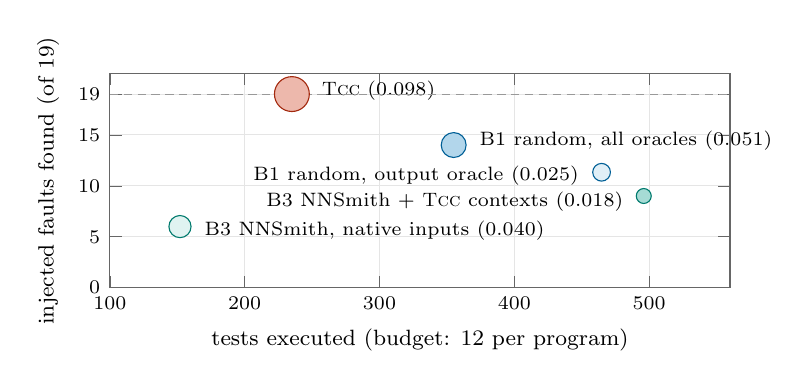
\begin{tikzpicture}
\begin{axis}[
    tccaxis, width=0.78\linewidth, height=4.3cm,
    xmin=100, xmax=560, ymin=0, ymax=21,
    xlabel={tests executed (budget: 12 per program)}, ylabel={injected faults found (of 19)},
    ytick={0,5,10,15,19},
    xmajorgrids,
    clip=false,
]
  %% x = tests, y = faults, radius ~ sqrt(test efficiency)
  \addplot[only marks, mark=*, mark size=6.3pt, draw=tolred!80!black, fill=tolred!35] coordinates {(235,19)};
  \addplot[only marks, mark=*, mark size=4.5pt, draw=tolblue!80!black, fill=tolblue!30] coordinates {(355,14)};
  \addplot[only marks, mark=*, mark size=3.2pt, draw=tolblue!80!black, fill=tolblue!12] coordinates {(464.7,11.33)};
  \addplot[only marks, mark=*, mark size=4.0pt, draw=tolteal!80!black, fill=tolteal!12] coordinates {(152,6)};
  \addplot[only marks, mark=*, mark size=2.7pt, draw=tolteal!80!black, fill=tolteal!35] coordinates {(496,9)};
  \node[anchor=west, font=\scriptsize] at (axis cs:250,19.3) {\tool (0.098)};
  \node[anchor=west, font=\scriptsize] at (axis cs:367,14.4) {B1 random, all oracles (0.051)};
  \node[anchor=east, font=\scriptsize] at (axis cs:455,11.0) {B1 random, output oracle (0.025)};
  \node[anchor=west, font=\scriptsize] at (axis cs:163,5.6) {B3 NNSmith, native inputs (0.040)};
  \node[anchor=east, font=\scriptsize] at (axis cs:488,8.4) {B3 NNSmith + \tool contexts (0.018)};
  \draw[black!40, densely dashed] (axis cs:100,19) -- (axis cs:560,19);
\end{axis}
\end{tikzpicture}
\caption{RQ2: faults found against tests executed under the same harness, oracles, and budget. Marker area is
proportional to test efficiency (unique failure clusters per executed test, in parentheses). B1 values are means
over three seeds.}
\label{fig:rq2}
\end{figure}


Figure~\ref{fig:rq2} plots, for a budget of 12 tests per program, the injected faults found against the tests
executed. Random generation with the output-only oracle that is customary in differential testing finds 11.3 of
19 faults (mean of three seeds) in 465 tests, 19\% of which are invalid; giving it all seven observables raises
it to 14, so one third of the gap is due to the oracle and two thirds to the choice of factors. NNSmith's
models expose no Python-level factors, so even with our contexts added detection stays at 9. \tool finds all 19 faults in 235 tests, with 16 invalid
contexts, and raises no alarm on the unmodified compiler. An ablation that enables the analysis layers
cumulatively (Figure~\ref{fig:rq3}) raises detection from 7 to 19 while the number of invalid tests falls from
109 to 16; alias facts and context sequences account for 9 of the 12 additional detections. Six faults require
a warm artifact: a cold-only comparison finds none of them in 148 tests, random sequences find 5, and
\scs-guided sequences find all 6 with 40\% fewer tests (Figure~\ref{fig:rq4}). Against the real compiler the
same sequences and 29 cross-process cache cases revealed no stale artifact. On the 193 mined reproducers
(Figure~\ref{fig:rq1-history}), detection of open issues stays at 41\% across PyTorch~2.10 and~2.14 while
detection of closed issues drops from 41\% to 13\%, which yields 35 verified buggy/fixed pairs.

%% Figure: lollipop chart for cache/specialization faults + test counts as annotated bars.
\begin{figure}[t]
\centering
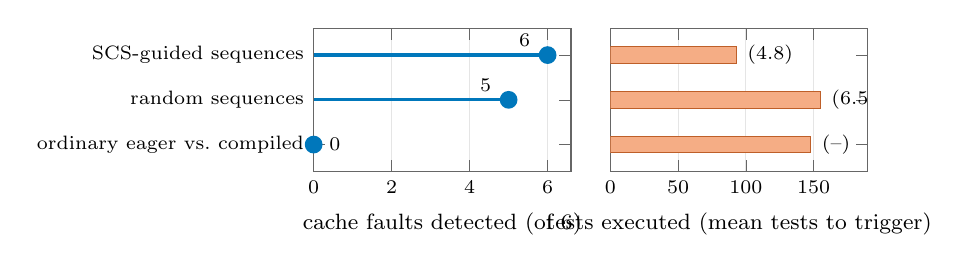
\begin{tikzpicture}
\begin{groupplot}[
    group style={group size=2 by 1, horizontal sep=0.5cm, y descriptions at=edge left},
    tccaxis, height=3.4cm,
    ytick={1,2,3},
    yticklabels={ordinary eager vs.\ compiled, random sequences, \scs-guided sequences},
    ymin=0.4, ymax=3.6, ymajorgrids=false, xmajorgrids,
]
  \nextgroupplot[width=0.40\linewidth, xmin=0, xmax=6.6, xtick={0,2,4,6}, xlabel={cache faults detected (of 6)}]
    \addplot[xcomb, very thick, tolblue, mark=*, mark size=2.6pt] coordinates {(0,1) (5,2) (6,3)};
    \node[font=\scriptsize, anchor=west] at (axis cs:0.15,1) {0};
    \node[font=\scriptsize, anchor=east] at (axis cs:4.8,2.32) {5};
    \node[font=\scriptsize, anchor=east] at (axis cs:5.8,3.32) {6};
  \nextgroupplot[width=0.40\linewidth, xmin=0, xmax=190, xlabel={tests executed (mean tests to trigger)}]
    \addplot[xbar, bar width=6pt, fill=tolorange!60, draw=tolorange!80!black] coordinates {(148,1) (155,2) (93,3)};
    \node[font=\scriptsize, anchor=west] at (axis cs:149,1) {(--)};
    \node[font=\scriptsize, anchor=west] at (axis cs:156,2) {(6.5)};
    \node[font=\scriptsize, anchor=west] at (axis cs:94,3) {(4.8)};
\end{groupplot}
\end{tikzpicture}
\caption{RQ4: the six faults that need a warm artifact. A cold-only comparison cannot observe them; \scs guidance
finds all six with fewer tests than random sequences.}
\label{fig:rq4}
\end{figure}

%% Figure: ablation -- faults detected (step line) and valid/invalid tests (stacked bars).
\begin{figure}[t]
\centering
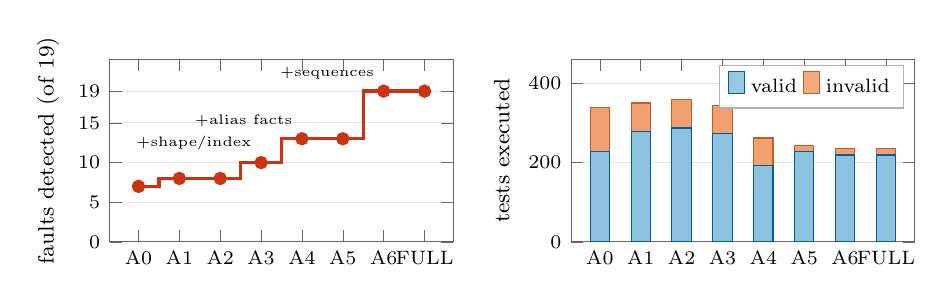
\begin{tikzpicture}
\begin{groupplot}[
    group style={group size=2 by 1, horizontal sep=1.5cm},
    tccaxis, width=0.49\linewidth, height=3.9cm,
    symbolic x coords={A0,A1,A2,A3,A4,A5,A6,FULL},
    xtick=data, x tick label style={font=\scriptsize},
]
  \nextgroupplot[ymin=0, ymax=23, ylabel={faults detected (of 19)}, ytick={0,5,10,15,19}]
    \addplot[const plot mark mid, very thick, tolred, mark=*, mark size=1.8pt]
      coordinates {(A0,7) (A1,8) (A2,8) (A3,10) (A4,13) (A5,13) (A6,19) (FULL,19)};
    \node[font=\tiny, anchor=south east] at (axis cs:A3,10.3) {+shape/index};
    \node[font=\tiny, anchor=south east] at (axis cs:A4,13.3) {+alias facts};
    \node[font=\tiny, anchor=south east] at (axis cs:A6,19.3) {+sequences};
  \nextgroupplot[ybar stacked, bar width=7pt, ymin=0, ymax=460, ylabel={tests executed},
                 legend pos=north east, legend columns=2]
    \addplot[fill=tolblue!45, draw=tolblue!80!black] coordinates
      {(A0,229) (A1,279) (A2,287) (A3,274) (A4,193) (A5,228) (A6,219) (FULL,219)};
    \addplot[fill=tolorange!70, draw=tolorange!80!black] coordinates
      {(A0,109) (A1,71) (A2,71) (A3,69) (A4,69) (A5,16) (A6,16) (FULL,16)};
    \legend{valid, invalid}
\end{groupplot}
\end{tikzpicture}
\caption{RQ3: cumulative ablation of the analysis layers (A0: dynamic random contexts; A1: tensor metadata;
A2: flow-sensitive dependencies; A3: shape--index relations; A4: alias and mutation facts; A5: \scs pruning;
A6: context sequences). Detection rises while the number of tests, and in particular of invalid tests, falls.}
\label{fig:rq3}
\end{figure}

%% Figure: slope chart of detection rates on mined issue reproducers across versions.
\begin{figure}[t]
\centering
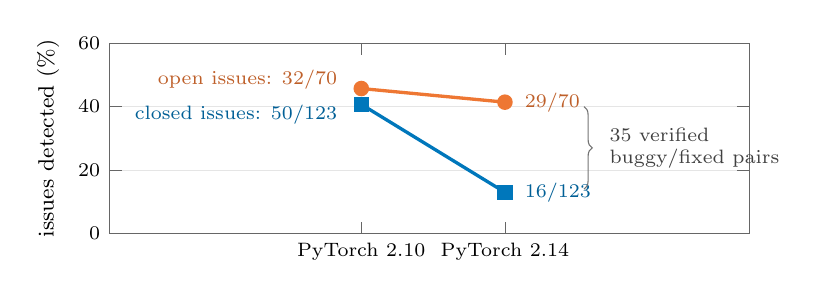
\begin{tikzpicture}
\begin{axis}[
    tccaxis, width=0.8\linewidth, height=4.0cm,
    xmin=-0.75, xmax=3.7, ymin=0, ymax=60,
    xtick={1,2}, xticklabels={PyTorch 2.10, PyTorch 2.14},
    ylabel={issues detected (\%)},
    clip=false,
]
  \addplot[tolorange, very thick, mark=*, mark size=2.2pt] coordinates {(1,45.7) (2,41.4)};
  \addplot[tolblue, very thick, mark=square*, mark size=2.2pt] coordinates {(1,40.7) (2,13.0)};
  \node[anchor=east, font=\scriptsize, tolorange!80!black] at (axis cs:0.9,48.5) {open issues: 32/70};
  \node[anchor=east, font=\scriptsize, tolblue!80!black] at (axis cs:0.9,37.5) {closed issues: 50/123};
  \node[anchor=west, font=\scriptsize, tolorange!80!black] at (axis cs:2.07,41.4) {29/70};
  \node[anchor=west, font=\scriptsize, tolblue!80!black] at (axis cs:2.07,13.0) {16/123};
  \draw[black!55, decorate, decoration={brace, amplitude=3pt, mirror}] (axis cs:2.55,14) -- (axis cs:2.55,40);
  \node[anchor=west, font=\scriptsize, black!75, align=left] at (axis cs:2.66,27) {35 verified\\buggy/fixed pairs};
\end{axis}
\end{tikzpicture}
\caption{RQ1 on 193 reproducers mined from the PyTorch issue tracker, executed on the same Linux CPU image with
two PyTorch versions. Open issues remain detectable; closed issues stop being detected once their fix ships.}
\label{fig:rq1-history}
\end{figure}


\rqanswer{RQ5}{Under identical oracles and budget, the one-factor matrix finds 19 faults against 14 for random
generation and 9 for NNSmith with half the tests; on the real compiler, guards and caches were consistent, and
the defects of RQ6 were reached through the paths behind them.}

\subsection{RQ6: Defects in Current PyTorch Builds}
\label{sec:rq6}

\paragraph{Reports.} The sweeps on PyTorch~2.14 and nightly builds have produced 73 items to date
(Table~\ref{tab:bugs} lists the issues): 55 new issues, 15 comments that add members, platforms, or a
corrected root cause to existing issues, and 3 reports to the vendor of the C++ compiler that TorchInductor
uses on Windows, whose optimizer folds vector intrinsics that PyTorch's own vectorized kernels emit. Every
candidate passed the confirmation steps of Section~\ref{sec:phase3}, was reproduced on PyTorch~2.14 and on a
nightly build, on Windows and Linux (and on CUDA where applicable), and was searched in the issue tracker by
root-cause keywords before filing. By maintainer response, 14 are fixed or have a fix under review, 10 are
confirmed by a maintainer or reproduced by another contributor, 48 await a human response, and 1 was judged
expected behavior (a mutated captured constant that export accepts and AOTInductor rejects). By root cause, 58
lie in the compile pipeline, 10 outside it, and 5 in other compilers (JAX, Numba, and the three MSVC reports). Of the 58,
42 are silent, 14 are failures of programs that eager execution accepts, and 2 terminate the process; they
span TorchDynamo (18), TorchInductor (29), AOTAutograd (4), decompositions and meta kernels (5), and export and
AOTInductor (3). Every change to \tcompile passes a continuous-integration suite that already runs OpInfo-based compiler
tests, and the tracker is triaged daily by dedicated teams.

\begin{table}[t]
\caption{The 55 issues filed against PyTorch and two other compilers (identifiers anonymized), in order of filing.
\emph{Layer}: Dy = TorchDynamo, AOT = AOTAutograd / autograd tracing, De = decompositions and meta kernels,
In = TorchInductor, Ex = export / AOTInductor, Eg = eager kernel shared by the compiled path, Fx = \code{torch.fx},
DM = dispatch machinery, Ext = another compiler. \emph{Sym.}: S = silent inconsistency, F = failure of a program
that eager execution accepts, C = process crash. \emph{Fac.}: P = program-side factor, Q = path-side factor.
\emph{Obs.}: observable that detected it (V value, D metadata, I identity, E exception, S state, G gradient,
R precision reference, C process). \emph{St.}: F fixed or fix under review, C confirmed, P pending, R rejected.}
\label{tab:bugs}
\scriptsize
\setlength{\tabcolsep}{3pt}
\begin{tabular}{@{}rp{8.2cm}llllll@{}}
\toprule
ID & Inconsistency (eager vs.\ compiled) & Layer & Sym. & Fac. & Obs. & St. \\
\midrule
B1  & \code{linalg.pinv} / \code{matrix\_sqrth}: wrong gradient for complex inputs & AOT & S & P & G & P \\
B2  & \code{random.shuffle} / \code{sample} return the same result on every call & Dy & S & Q & V & F \\
B3  & \code{jvp} of \code{ldexp} terminates the interpreter under \ET & AOT & C & Q & C & P \\
B4  & arg-reduction index emitted with Python \code{**} in C++; compilation fails & In & F & Q & E & C \\
B5  & \code{new\_zeros(device="cpu")} returns a CUDA tensor & In & S & Q & D & C \\
B6  & \code{std} / \code{var}: NaN for $10^{30}$, zero value \emph{and zero gradient} for $10^{-30}$ & In & S & P & V & P \\
B7  & \code{jvp} of \code{quantile} / \code{addr}: internal assertion on every backend & Dy & F & Q & E & P \\
B8  & \code{ldexp} result dtype wrong in both directions & In & S & P & D & F \\
B9  & compiled autograd: \code{interpolate} backward hits an internal assertion & AOT & F & Q & E & P \\
B10 & f-string format specifier on a symbolic size: internal Dynamo error & Dy & F & Q & E & C \\
B11 & compiled \code{SGD.step}, \code{foreach=True}, complex parameters: lowering assertion & In & F & P & E & C \\
B12 & \code{interpolate} on an empty spatial dim returns NaNs (out-of-bounds read); eager raises & De & S & P & E & C \\
B13 & mutated captured tensor: export accepts, decomposition rejects, AOTInductor asserts & Ex & F & Q & E & R \\
B14 & \code{vector\_norm(ord=inf)} on an empty batch fails only for negative \code{dim} & De & F & P & E & F \\
B15 & \code{binary\_cross\_entropy} / \code{huber\_loss}: float32 result for half-precision inputs & In & S & P & D & P \\
B16 & \code{pdist} backward on zero rows: integer division by zero kills the process & Eg & C & P & C & F \\
B17 & \code{random.seed} inside the function is ignored on the first call & Dy & S & Q & V & F \\
B18 & named tuple \code{==} with tensor fields: \code{RecursionError} (Python 3.14 only) & Dy & F & Q & E & P \\
B19 & \code{bmm} under autotuning: missing symbol export in a C++ template (Windows) & In & F & Q & E & P \\
B20 & AOTInductor cannot package models returning \code{torch.return\_types.*} & Ex & F & Q & E & F \\
B21 & \code{lerp} of Boolean tensors with a 0-d weight fails to compile & De & F & P & E & F \\
B22 & \code{sum} / \code{prod} with \code{dtype=torch.bool}: C++ error / assertion & In & F & P & E & P \\
B23 & \code{addmm} with a 0-d bias under autotuning: \code{IndexError} in lowering & In & F & Q & E & F \\
B24 & \code{var\_mean} / \code{std\_mean} of an empty tensor: mean is 0 instead of NaN & In & S & P & V & F \\
B25 & \code{channel\_shuffle} loses the \code{channels\_last} layout & In & S & P & D & C \\
B26 & \code{str(KeyError(k))} loses the quotes that CPython adds & Dy & S & P & V & F \\
B27 & \code{abs(complex, out=float64)} rejected by the meta kernel & De & F & P & E & C \\
C1  & in-place-modification check lost for a saved input view: silent wrong gradients & AOT & S & P & G & F \\
C2  & \code{adaptive\_max\_pool3d} backward wrong for \code{channels\_last\_3d} (eager kernel) & Eg & S & P & G & C \\
C3  & a changing Python float argument is baked into the cached graph & Dy & S & Q & V & P \\
C7  & Numba: \code{remainder} of \code{MIN\_INT} by $-1$ kills the process & Ext & C & -- & C & P \\
C8  & \code{x * 1} / \code{x + 0} as a graph output return the input object itself & In & S & P & I & C \\
C9  & \code{torch.fx} codegen: \code{operator.pow(-2, x)} emitted as \code{-2**x} & Fx & S & P & V & F \\
C10 & floating-point floor division off by one (\code{1.0 // 0.1} gives 10) & In & S & P & V & C \\
C11 & closure mutations in methods of a locally defined class are dropped & Dy & S & P & S & F \\
C12 & JAX: \code{gcd} / \code{lcm} hang on the integer minimum & Ext & C & -- & C & F \\
C13 & compiled NumPy code: \code{fix}, \code{cbrt}, \code{clip}, \code{sign} return wrong values & Dy & S & P & V & P \\
C14 & vectorized \code{remainder}: NaN for an infinite divisor, 0 for large quotients & In & S & P & V & P \\
C16 & \code{round(SymInt, -1)} is the identity & Dy & S & P & V & P \\
C17 & NaN self-comparison of an \code{.item()} value folded to a constant & Dy & S & P & V & P \\
C20 & compiled NumPy code: dtype and shape rules differ (\code{cumsum}, \code{square}, \code{median}) & Dy & S & P & D & P \\
C22 & \code{clamp(int8, -1000, 1000)} returns $-24$: bounds wrapped into int8 & In & S & P & V & P \\
C24 & \code{torch.fx}: parameters named \code{nan} / \code{inf} shadow float constants & Fx & S & P & V & P \\
C27 & \code{GraphModule} pickle round trip turns in-place nodes into out-of-place ones & Fx & S & Q & S & P \\
C29 & \code{any(uint8)} returns \code{bool} instead of \code{uint8} & In & S & P & D & P \\
C32 & complex \code{pinv} / \code{polar} / \code{matrix\_sqrth} wrong under any dispatch mode & DM & S & Q & V & P \\
C34 & \code{avg\_pool} backward with \code{ceil\_mode}: full kernel size as divisor for the last window & In & S & P & G & P \\
C35 & \code{erfinv} loses four digits near $\pm 1$ & In & S & P & R & P \\
C36 & vectorized float64 \code{acosh} overflows above $1.3\times10^{154}$ & In & S & P & V & P \\
C37 & 134 operators compute on dtypes the eager kernel rejects (418 pairs) & In & S & P & E & P \\
C40 & vectorized float32 \code{erf} returns 0 below $10^{-7}$; \code{atanh} returns 0 below $\epsilon$ & In & S & P & R & P \\
C41 & \code{OrderedDict.move\_to\_end} on an input dictionary is dropped & Dy & S & Q & S & P \\
C42 & a generator that leaves the compiled region returns as an exhausted tuple iterator & Dy & S & Q & I & P \\
C44 & \code{IndexError} from a tensor operator bypasses the program's \code{except} clause & Dy & S & P & E & P \\
C46 & AOTInductor runner destroyed after a run: access violation (Windows, OpenMP workers still spinning) & Ex & C & Q & C & P \\
\bottomrule
\end{tabular}
\end{table}


\paragraph{Findings over time.} The first 27 issues (B1--B27) were found with default paths; 14 of them are
failures of programs that eager execution accepts. The issues found after the path factors and the
metadata-derived factors were added (C1--C46) are silent in 26 of 28 cases and include the four Dynamo defects
of RQ1, the identity defect C8, the 134-operator family C37, and the three accuracy defects. The maintainers'
own umbrella issue on lost validation, opened during the study, lists several of our reports as members.

%% Figure: (a) heatmap factor group x layer over the 68 PyTorch items, (b) stacked bars symptom per layer.
\newcommand{\hcell}[3]{% x, y, count
  \pgfmathsetmacro{\shade}{min(100, 12 + 7*#3)}
  \ifnum#3>0
    \fill[tolblue!\shade!white] (#1-0.5,#2-0.5) rectangle (#1+0.5,#2+0.5);
    \node[font=\scriptsize, text=\ifnum#3>7 white\else black\fi] at (#1,#2) {#3};
  \else
    \node[font=\scriptsize, black!35] at (#1,#2) {$\cdot$};
  \fi}
\begin{figure}[t]
\centering
\begin{minipage}[b]{0.58\linewidth}
\centering
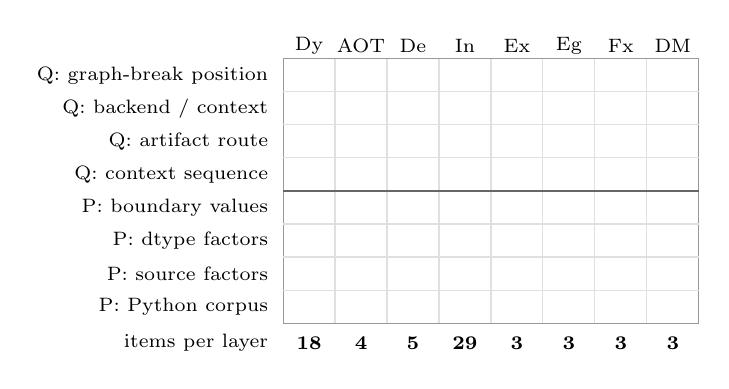
\begin{tikzpicture}[x=0.66cm, y=0.42cm]
  %% columns: 1 Dy, 2 AOT, 3 De, 4 In, 5 Ex, 6 Eg, 7 Fx, 8 DM ; rows top->bottom 8..1
  \foreach \x/\lab in {1/Dy, 2/AOT, 3/De, 4/In, 5/Ex, 6/Eg, 7/Fx, 8/DM} \node[font=\scriptsize] at (\x,8.9) {\lab};
  \foreach \y/\lab in {8/{Q: graph-break position}, 7/{Q: backend / context}, 6/{Q: artifact route},
                       5/{Q: context sequence}, 4/{P: boundary values}, 3/{P: dtype factors},
                       2/{P: source factors}, 1/{P: Python corpus}}
    \node[font=\scriptsize, anchor=east] at (0.4,\y) {\lab};
  %% data (findings.csv, items with a PyTorch layer; cross-target items excluded)
  \hcell{1}{8}{3}\hcell{2}{8}{0}\hcell{3}{8}{0}\hcell{4}{8}{0}\hcell{5}{8}{0}\hcell{6}{8}{0}\hcell{7}{8}{0}\hcell{8}{8}{0}
  \hcell{1}{7}{3}\hcell{2}{7}{2}\hcell{3}{7}{0}\hcell{4}{7}{5}\hcell{5}{7}{0}\hcell{6}{7}{0}\hcell{7}{7}{0}\hcell{8}{7}{3}
  \hcell{1}{6}{0}\hcell{2}{6}{0}\hcell{3}{6}{0}\hcell{4}{6}{0}\hcell{5}{6}{3}\hcell{6}{6}{0}\hcell{7}{6}{1}\hcell{8}{6}{0}
  \hcell{1}{5}{4}\hcell{2}{5}{0}\hcell{3}{5}{0}\hcell{4}{5}{0}\hcell{5}{5}{0}\hcell{6}{5}{0}\hcell{7}{5}{0}\hcell{8}{5}{0}
  \hcell{1}{4}{1}\hcell{2}{4}{0}\hcell{3}{4}{3}\hcell{4}{4}{13}\hcell{5}{4}{0}\hcell{6}{4}{2}\hcell{7}{4}{0}\hcell{8}{4}{0}
  \hcell{1}{3}{1}\hcell{2}{3}{1}\hcell{3}{3}{2}\hcell{4}{3}{10}\hcell{5}{3}{0}\hcell{6}{3}{0}\hcell{7}{3}{0}\hcell{8}{3}{0}
  \hcell{1}{2}{2}\hcell{2}{2}{1}\hcell{3}{2}{0}\hcell{4}{2}{1}\hcell{5}{2}{0}\hcell{6}{2}{1}\hcell{7}{2}{0}\hcell{8}{2}{0}
  \hcell{1}{1}{4}\hcell{2}{1}{0}\hcell{3}{1}{0}\hcell{4}{1}{0}\hcell{5}{1}{0}\hcell{6}{1}{0}\hcell{7}{1}{2}\hcell{8}{1}{0}
  \draw[black!40] (0.5,0.5) rectangle (8.5,8.5);
  \foreach \x in {1.5,2.5,...,7.5} \draw[black!12] (\x,0.5) -- (\x,8.5);
  \foreach \y in {1.5,2.5,...,7.5} \draw[black!12] (0.5,\y) -- (8.5,\y);
  \draw[black!60, thick] (0.5,4.5) -- (8.5,4.5);
  %% marginals
  \foreach \x/\s in {1/18, 2/4, 3/5, 4/29, 5/3, 6/3, 7/3, 8/3} \node[font=\scriptsize\bfseries] at (\x,-0.1) {\s};
  \node[font=\scriptsize, anchor=east] at (0.4,-0.1) {items per layer};
\end{tikzpicture}
\subcaption{Items by factor group (Q = path side, P = program side) and layer.}
\end{minipage}\hfill
\begin{minipage}[b]{0.40\linewidth}
\centering
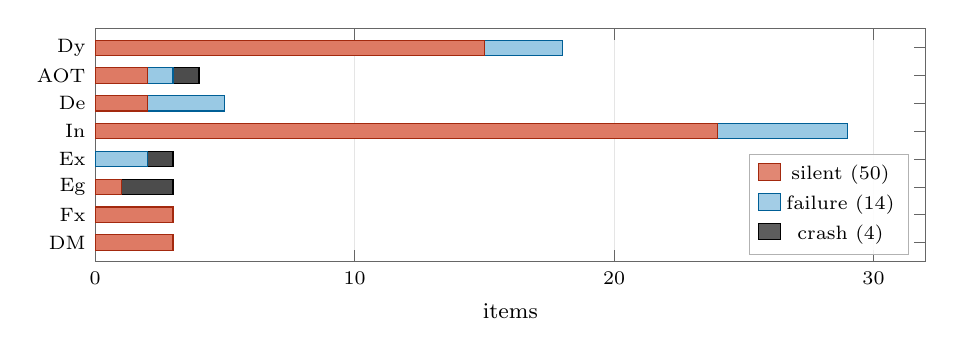
\begin{tikzpicture}
\begin{axis}[
    tccaxis, width=\linewidth, height=4.55cm,
    xbar stacked, bar width=5.5pt,
    ytick={1,2,3,4,5,6,7,8}, yticklabels={DM, Fx, Eg, Ex, In, De, AOT, Dy},
    xmin=0, xmax=32, xtick={0,10,20,30}, xlabel={items}, ymajorgrids=false, xmajorgrids,
    legend style={at={(0.98,0.03)}, anchor=south east}, legend columns=1,
]
  \addplot[fill=tolred!65, draw=tolred!80!black] coordinates {(3,1) (3,2) (1,3) (0,4) (24,5) (2,6) (2,7) (15,8)};
  \addplot[fill=tolblue!40, draw=tolblue!80!black] coordinates {(0,1) (0,2) (0,3) (2,4) (5,5) (3,6) (1,7) (3,8)};
  \addplot[fill=black!70, draw=black] coordinates {(0,1) (0,2) (2,3) (1,4) (0,5) (0,6) (1,7) (0,8)};
  \legend{silent (50), failure (14), crash (4)}
\end{axis}
\end{tikzpicture}
\subcaption{Symptoms per layer.}
\end{minipage}
\caption{RQ6: distribution of the 68 PyTorch items (issues and comments) by factor group, layer, and symptom.
Layer abbreviations as in Table~\ref{tab:bugs}; the five cross-compiler items are omitted.}
\label{fig:rq5}
\end{figure}


\paragraph{Cost and negative results.} The compile-based campaigns on default paths were the most expensive and the least productive:
about 2{,}800 programs and 45{,}000 differential tests on default paths produced one new defect, the
fabricated mean of Figure~\ref{fig:motivation}b. The path-side and metadata-derived analyzers produced the
remaining defects at a fraction of the cost. Table~\ref{tab:negative} lists the factor families that found
nothing new; they bound the claim of this paper and tell developers where consistency already holds.


\rqanswer{RQ6}{\tool led to 73 reports against PyTorch~2.14 and nightly builds and two other compilers; 14
are fixed or have a fix under review and 10 are confirmed. Of the 58 pipeline findings 42 are silent, and none
appears with a contiguous float32 tensor on the default path.}

\section{Discussion}
\label{sec:discussion}

\subsection{Lessons}

\paragraph{Varying the compilation.} None of the 58 pipeline findings occurs with a contiguous
float32 tensor on the default path, and 20 of them occur only when the path changes. RQ1 isolates this
effect: with program set, inputs, and oracle held fixed on a corpus already run under three configurations, one
additional path factor produced two defects within minutes. The explanation lies in the code
that each factor reaches. A graph break makes every live local an input of a resume function, so the machinery
that reconstructs Python objects and replays side effects is exercised for objects that a single-graph run
never reconstructs. A dispatch mode routes composite operators through a path on which conjugate views are
materialized lazily. A packaged runtime has a lifetime that the just-in-time runtime does not have. Program
diversity does not reach this code because the program cannot select the path.

\paragraph{Seeds written after a finding.} Both corpus additions of RQ1 followed a finding. The first, written
for the mechanisms behind C41 and C42, re-found those two under the break factor and exposed C44 through its
exception-flow programs on the unmodified path; the second, written for C44, delimited it without adding a defect. A batch of 34 generic programs written before any finding produced nothing new.

\paragraph{Lost validation.} Nine findings return a value where eager execution raises, and 13 raise where
eager execution returns. The first group is not harmless: C37 computes convolutions on Boolean inputs and
softmax on integers with results that no eager kernel defines, and the maintainers opened an umbrella issue on
lost validation during the study. An oracle that ignores exceptions, or a harness that discards every context in
which eager execution raises, misses this class. In the historical benchmark, fourteen open issues ran
zero tests until the harness stopped discarding such seeds.

\paragraph{Reference strength.} Three accuracy findings (C35, C36, C40) are invisible in an
eager-versus-compiled comparison at ordinary inputs and appeared only against a multi-precision reference next to
singularities. A float64 reference separates rounding noise from wrong results for
well-conditioned computations but not for ill-conditioned ones: five closed historical issues that \tool still
flags had been judged intended behavior because a legal re-association is amplified by a later operator.
Such findings are annotated for manual review; condition-aware suppression is future work.

\subsection{Threats to Validity}
\label{sec:threats}

\paragraph{Internal validity.} Harness defects can appear as compiler defects. Two occurred during the study: a
wrapper that compiled the wrong callee, and a sample generator whose \code{no\_grad} finalizer ran inside a
later trace and inserted a grad-mode node into exported graphs. Every candidate is therefore confirmed with a stand-alone script that does not
import \tool, in a fresh interpreter, on two PyTorch versions and two operating systems, and every report is
re-verified from its text before filing. Injected faults may not represent real defects, so the evaluation
also uses mined issues and defects found in current builds.

\paragraph{Construct validity.} A differential oracle detects a divergence and does not decide which side is wrong; ten findings had their root cause outside the pipeline and are counted
separately. Layer attribution was validated against the location of 13 fixes, which biases the check
toward defects that were easy to fix. The maintainer-response counts reflect the tracker at the time of writing;
most path-factor items were filed in the last days before submission. The comparison in RQ5 covers random
generation and NNSmith; TorchProbe, the closest tool, could not be run against our subject.

\paragraph{External validity.} The implementation targets \tcompile; the factor model needs only an eager
reference, pipeline switches, and selectable layers, which other AI compiler stacks also offer but which we have
not evaluated. Most experiments ran on CPUs; the T4 runs confirmed the platform-independent
defects and found CUDA-specific members of C37, but Triton code generation is covered less densely than C++
code generation, and C46 is specific to Windows.
\clearpage

\section{Related Work}
\label{sec:related}

\paragraph{Testing AI compiler stacks.} Empirical studies show that DL compiler defects concentrate in
high-level optimization and lowering and that a large share produce wrong results rather than
crashes~\cite{DBLP:conf/sigsoft/ShenM0TCC21,DBLP:journals/tpds/LiLLSYYLGYQ21}. Generators address this from the input side. NNSmith~\cite{DBLP:conf/asplos/LiuLRTLPZ23} and
NeuRI~\cite{DBLP:conf/sigsoft/0004PW023} synthesize valid and diverse computation graphs from operator constraints, GenCoG~\cite{DBLP:conf/issta/WangNMCWB023}
does so with a constraint DSL for TVM, HirGen~\cite{DBLP:conf/issta/MaS00C23} targets high-level IR, Tzer~\cite{DBLP:journals/pacmpl/LiuWYDZ22} mutates TVM's
low-level IR together with pass sequences, and MLIRSmith~\cite{DBLP:conf/kbse/WangCXLWSZ23} generates MLIR programs.
WhiteFox~\cite{DBLP:journals/pacmpl/YangDLY0J024} lets a language model read optimization source code to produce inputs that trigger it.
Xiao \etal~\cite{DBLP:conf/sigmetrics/XiaoLYPW22} apply metamorphic relations to compiled models. TorchProbe~\cite{DBLP:conf/aplas/SuGPS23} is closest
to our subject: it rewrites Python programs with semantics-preserving transformations that introduce dynamic
language features and compares the variants under PyTorch~2. These techniques decide \emph{which program} to
compile, and each of them compiles it along one path. \tool is orthogonal: for a given program it varies the
compilation (graph-break position, backend layer, execution context, artifact route) and the program-side
factors the program reads, one at a time, and compares identity, state, exception routing, gradients, metadata,
and process survival besides values. TorchProbe's transformations and the cold/warm cache comparison of
AlignGuard\footnote{arXiv preprint, 2026.} are single members of this factor space; the configuration
relations of~\cite{DBLP:conf/sigmetrics/XiaoLYPW22} vary the model rather than the compiler. Equivalence modulo
inputs~\cite{DBLP:conf/pldi/LeAS14} and metamorphic testing~\cite{DBLP:journals/csur/ChenKLPTTZ18,DBLP:journals/tse/SeguraFSC16} supply the
form of our relation, observable equality under a semantics-preserving change; the change here is to the
compilation rather than to the program.

\paragraph{Testing deep learning libraries.} CRADLE~\cite{DBLP:conf/icse/PhamLQT19}, Audee~\cite{DBLP:conf/kbse/GuoXLZLLS20}, LEMON~\cite{DBLP:conf/sigsoft/WangYCLZ20}, and
Muffin~\cite{DBLP:conf/icse/GuLZ022} compare models across frameworks or back ends. FreeFuzz~\cite{DBLP:conf/icse/WeiDYZ22} mines API
invocations from documentation, tests, and models; DeepREL~\cite{DBLP:conf/sigsoft/DengYWZ22} infers relations between APIs;
DocTer~\cite{DBLP:conf/issta/XieLKP0ZG22} and ACETest~\cite{DBLP:conf/issta/ShiXLLYYSCH23} extract input constraints from documentation and validation
code; TitanFuzz~\cite{DBLP:conf/issta/DengXPY023} and FuzzGPT~\cite{DBLP:conf/icse/DengXYZY024} generate API programs with language models;
Predoo~\cite{DBLP:conf/issta/ZhangSFLLCWC21} studies operator precision; and $\nabla$Fuzz~\cite{DBLP:conf/icse/YangDYTLZ23} differentially tests automatic
differentiation. Studies of framework bugs~\cite{DBLP:conf/sigsoft/IslamNPR19,DBLP:journals/tosem/ChenLSJL23,DBLP:conf/kbse/GuoCXMHLLZL19} and of silent
bugs~\cite{DBLP:journals/ese/TambonNAKA24} motivate oracles beyond crashes. \tool borrows the seeds these communities created
(OpInfo is PyTorch's counterpart to a mined API corpus) but asks a different question: not whether an API is
correct, but whether its compiled execution agrees with its eager execution in every observable, including under
forward-mode, compiled, and complex-valued differentiation, where our sweeps found defects (B1, B3, B7, B9) that
eager-only AD testing cannot reach.

\paragraph{Compiler testing and validation.} Differential testing~\cite{DBLP:journals/dtj/McKeeman98}, random program generation
with Csmith~\cite{DBLP:conf/pldi/YangCER11} and YARPGen~\cite{DBLP:journals/pacmpl/LivinskiiBR20}, and equivalence modulo inputs~\cite{DBLP:conf/pldi/LeAS14} are the foundations
of compiler testing~\cite{DBLP:journals/csur/ChenPPXZHZ20}; metamorphic testing~\cite{DBLP:journals/tse/SeguraFSC16,DBLP:journals/csur/ChenKLPTTZ18} and
the oracle problem~\cite{DBLP:journals/tse/BarrHMSY15} frame what can be compared. For JIT compilers, Artemis~\cite{DBLP:conf/sosp/Li00S23} explores
the space of compilation decisions and JIT-Picking~\cite{DBLP:conf/ccs/BernhardSSBH22} compares interpreter and JIT executions of
JavaScript engines; our layered execution likewise uses the non-optimizing tier as a reference, with three intermediate tiers. Test-case reduction by delta
debugging~\cite{DBLP:journals/tse/ZellerH02} and C-Reduce~\cite{DBLP:conf/pldi/RegehrCCEEY12} inspires our minimizer, which additionally uses the static
slice of the triggering factor. Verified compilation~\cite{DBLP:journals/cacm/Leroy09} and translation
validation~\cite{DBLP:conf/tacas/PnueliSS98,DBLP:conf/pldi/LopesLHLR21} establish consistency by proof; they do not yet scale to an AI compiler stack
with data-dependent guards, code generation through C++ and Triton, and caches, which is why a testing approach
with strong oracles is the practical option today.

\paragraph{Source--artifact consistency and the software supply chain.} Thompson's trusting-trust
attack~\cite{DBLP:journals/cacm/Thompson84} is the classical example of an artifact that departs from its reviewed source.
Reproducible builds~\cite{DBLP:journals/software/LambZ22}, in-toto~\cite{DBLP:conf/uss/Torres-AriasAKC19}, and Sigstore~\cite{DBLP:conf/ccs/NewmanMT22} secure the path from
source to artifact against tampering, and taxonomies of supply-chain attacks~\cite{DBLP:conf/dimva/OhmPS020,DBLP:conf/sp/LadisaPMB23} catalog
how that path is abused. These defenses establish \emph{who} built an artifact and \emph{from what}, not that a benign compiler
preserved the semantics of benign source. \tool addresses that gap for AI compiler stacks~\cite{DBLP:conf/nips/PaszkeGMLBCKLGA19,DBLP:conf/asplos/AnselYHGJVBBBBC24,DBLP:conf/osdi/ChenMJZYSCWHCGK18}, where the artifact is generated, specialized, and
cached at run time on the user's machine.

\section{Conclusion}
\label{sec:conclusion}

A compiled deep learning program should behave like the Python source its developers reviewed on every path
the compiler may take. \tool tests this property by varying the compilation rather than only
the program: graph-break positions, backend layers, execution contexts, and artifact routes are enumerated
and changed one at a time, alongside program-side factors derived from the source and from operator metadata,
and every execution is compared on seven observables. Reports against PyTorch~2.14 and nightly builds number 73 items, of which 14 are fixed or have a fix under review and 10 are confirmed. The path
dimension accounts for 20 of the 58 pipeline findings and for both defects found on a corpus that program-only
testing had already covered; observables beyond the output value account for 39. Guards, caches, compile composition,
autocast, and the values of the export route were consistent. Future work will add condition-aware numerical
oracles, denser coverage of the Triton path, and ports of the factor model to other AI compiler stacks.

\section*{Data Availability}
The implementation of \tool, the benchmarks, the sweep records, the classification of the 73 reports, and the
stand-alone reproducer of every report are available in an anonymized artifact.


\bibliographystyle{ACM-Reference-Format}
\bibliography{bib/references}

\end{document}
